\documentclass[10pt,preprint2]{aastex}
\usepackage[a4paper,asymmetric,left=0.75in,right=0.75in,top=0.75in,bottom=0.75in]{geometry}
\AtBeginDocument{\newgeometry{asymmetric,left=0.75in,right=0.75in,top=0.75in,bottom=0.75in}\hoffset=0pt\setlength{\columnsep}{0.3in}\pagestyle{fancy}\fancyhf{}\fancyhead[L]{\small ASTRON 121 Radio Astronomy Laboratory}\fancyhead[R]{\small Lab 3}\fancyfoot[C]{\thepage}}
\usepackage{amsmath, amsfonts, amssymb}
\usepackage{hyperref}
\usepackage{graphicx}
\usepackage{booktabs}
\usepackage{fancyhdr}
\setlength{\headheight}{11pt}
\addtolength{\topmargin}{-0.16pt}
\usepackage{float}
\usepackage{stfloats}
\usepackage{placeins}
\let\tablenum\relax
\usepackage{siunitx}
\usepackage{tikz}
\usetikzlibrary{arrows.meta,positioning,calc,decorations.pathmorphing,decorations.pathreplacing,patterns,fit}

\makeatletter\def\frontmatter@abstractheading{}\makeatother
\renewcommand{\abstractname}{}

\begin{document}

\title{Interferometric X-Band Observations of the Sun}
\author{Jun Rui Ting \\ \today\vspace{-2.5\baselineskip}}

\begin{abstract}
We present interferometric observations of the Sun at 10.45~GHz using the two-dish correlating interferometer at the New Campbell Hall (NCH) observatory, Berkeley. Five independent baseline-determination methods---including short-time Fourier transform (STFT) fringe-frequency fitting, delay-spectrum analysis, nonlinear least-squares (NLS) fringe fitting, and a two-dimensional brute-force grid search---are applied to horizon-to-horizon drift-scan data comprising 8226 visibility integrations across 285 spectral channels. The adopted baseline, $b_{\mathrm{ew}} = 15.1148 \pm 0.0000$~m (formal) and $b_{\mathrm{ns}} = 1.4746 \pm 0.0000$~m, is consistent with an independent iPhone LiDAR survey ($15.17 \pm 0.30$~m) at the $0.2\sigma$ level. The angular diameter of the Sun is measured from the Bessel-function (jinc) modulation of the fringe-amplitude envelope, yielding $D_\odot = 34.664 \pm 0.034'$ (statistical) $\pm\,3.38'$ (systematic), consistent with the 17~GHz radio reference of $32.55 \pm 0.05'$ \citep{Selhorst2004}. A non-zero sunspot floor $f \approx 0.033$ and a limb-brightening coefficient $\varepsilon \approx 2.0$ are detected, indicating an active region on the solar disk during the observation.

\vspace{2.5\baselineskip}
\end{abstract}

%%% ---------------------------------------------------------------
\section{Introduction}
\label{sec:intro}
%%% ---------------------------------------------------------------

Radio interferometry is the foundation of modern radio astronomy and the technique by which the event horizon of a supermassive black hole was first imaged. By correlating the signals from two or more spatially separated antennas, an interferometer achieves angular resolution determined not by the diameter of any single dish, but by its baseline separation. This principle underpins instruments from the Very Large Array (VLA) in New Mexico to the Event Horizon Telescope (EHT), a planet-scale array that achieves microarcsecond resolution \citep{TMS2017}.

In this work, we employ the two-dish X-band interferometer at the New Campbell Hall (NCH) observatory on the UC Berkeley campus to pursue three scientific objectives:
\begin{enumerate}
\item \textbf{Baseline calibration.} We determine the interferometer baseline vector $(b_{\mathrm{ew}}, b_{\mathrm{ns}})$ from the fringe data alone, using five independent methods, and compare the result with an external LiDAR survey.
\item \textbf{Solar diameter.} We measure the angular diameter of the Sun at a frequency of $\sim$10.45~GHz, where the emission is dominated by free--free (bremsstrahlung) radiation from the chromosphere. At centimetre wavelengths, the radio Sun is expected to appear several percent larger than the optical photosphere because the $\tau = 1$ surface lies a few thousand kilometres above the visible limb \citep{Dulk1985, Stix2002}.
\item \textbf{Active-region detection.} We search for the signature of unresolved sunspot emission as a non-zero floor in the visibility amplitude at the Bessel-function nulls.
\end{enumerate}

The interferometer operates at a sky frequency of approximately 10.45~GHz ($\lambda \approx 2.87$~cm), with a nearly east--west baseline of $b_{\mathrm{ew}} \approx 15$~m. A SNAP-board FX correlator digitises both signals at 500~Msps, cross-correlates them in 1024 spectral channels, and integrates for 1.25~s per visibility spectrum \citep{TMS2017}. The fringe pattern generated by the Earth's rotation encodes both the geometry of the baseline and the brightness distribution of the source; by analysing the fringe frequency, phase, and amplitude envelope, we extract both the baseline and the solar diameter from a single horizon-to-horizon drift scan.

The remainder of this report is organised as follows. Section~\ref{sec:theory} develops the theoretical framework: the geometric delay, the fringe equation, the local fringe frequency, the extended-source response via the van~Cittert--Zernike theorem, and the Bessel-function (jinc) visibility for a uniform disk. Section~\ref{sec:obs} describes the instrument and the observations. Section~\ref{sec:reduction} presents the data reduction pipeline, including the adaptive DC correction and fringe-frequency diagnostics. Section~\ref{sec:baseline} details seven baseline-determination methods and their comparison. Section~\ref{sec:diameter} presents the solar-diameter measurement using four complementary approaches. Section~\ref{sec:discussion} discusses the error budget, sunspot and limb-brightening characterisation, and the physical interpretation of the radio Sun. Section~\ref{sec:conclusions} summarises the main results.


%%% ---------------------------------------------------------------
\section{Background Theory}
\label{sec:theory}
%%% ---------------------------------------------------------------

A single radio dish of diameter $D$ has an angular resolution limited by diffraction to $\theta \sim \lambda/D$. At our observing wavelength of $\lambda = 2.87$~cm, a 1-metre dish resolves only $\sim$$1.6^\circ$---far too coarse to resolve the Sun's $\sim$$0.5^\circ$ disk, let alone finer structure. A 15-metre dish would be needed to match the Sun's angular size, and arcsecond-scale resolution would require a dish hundreds of metres across.

Interferometry circumvents this limitation. Instead of building one enormous aperture, we place two small dishes a distance $b$ apart---the \emph{baseline}---and correlate their signals. The correlated output is sensitive to angular structure on the scale $\theta \sim \lambda/b$, the same resolution a filled aperture of diameter $b$ would achieve, but without filling the aperture \citep{TMS2017}. For our 15-metre baseline at 2.87~cm, this corresponds to $\theta \sim 6.6'$---well matched to the solar diameter and sufficient to resolve its disk.

The key physical quantity the interferometer measures is the \emph{complex visibility} $V(u)$: the Fourier component of the sky brightness distribution at the spatial frequency $u = b_{\mathrm{proj}}/\lambda$, where $b_{\mathrm{proj}}$ is the projected baseline perpendicular to the line of sight. As the Earth rotates, the projected baseline changes continuously, so the interferometer samples a different spatial frequency at each moment. Over a full drift scan from horizon to horizon, a single baseline traces out an arc in the Fourier plane (the $uv$-plane), building up a one-dimensional slice through the Fourier transform of the source brightness. This is the principle of \emph{aperture synthesis}: by combining visibility measurements at many spatial frequencies, one can reconstruct the image of the source \citep{TMS2017, FomalontWright1974}.

For a point source, the visibility amplitude is constant and the phase oscillates with the changing geometric delay---this oscillation is the \emph{fringe}. For an extended source like the Sun, the visibility amplitude is modulated by the Fourier transform of the brightness distribution, producing characteristic nulls where the fringe spacing matches the source size (Section~\ref{sec:jinc}). The positions of these nulls encode the source diameter.

Figure~\ref{fig:interferometer} illustrates the geometry. Two dishes separated by baseline $b$ observe the Sun at an angle $\theta$ from the zenith. Plane wavefronts from the source arrive at the two dishes with a relative path delay $\tau_g$, which depends on the projected baseline and changes as the Earth rotates. The signals are brought together in the SNAP FX correlator, which cross-multiplies the Fourier-transformed voltages to produce the complex visibility spectrum.

\begin{figure*}[t]
\centering
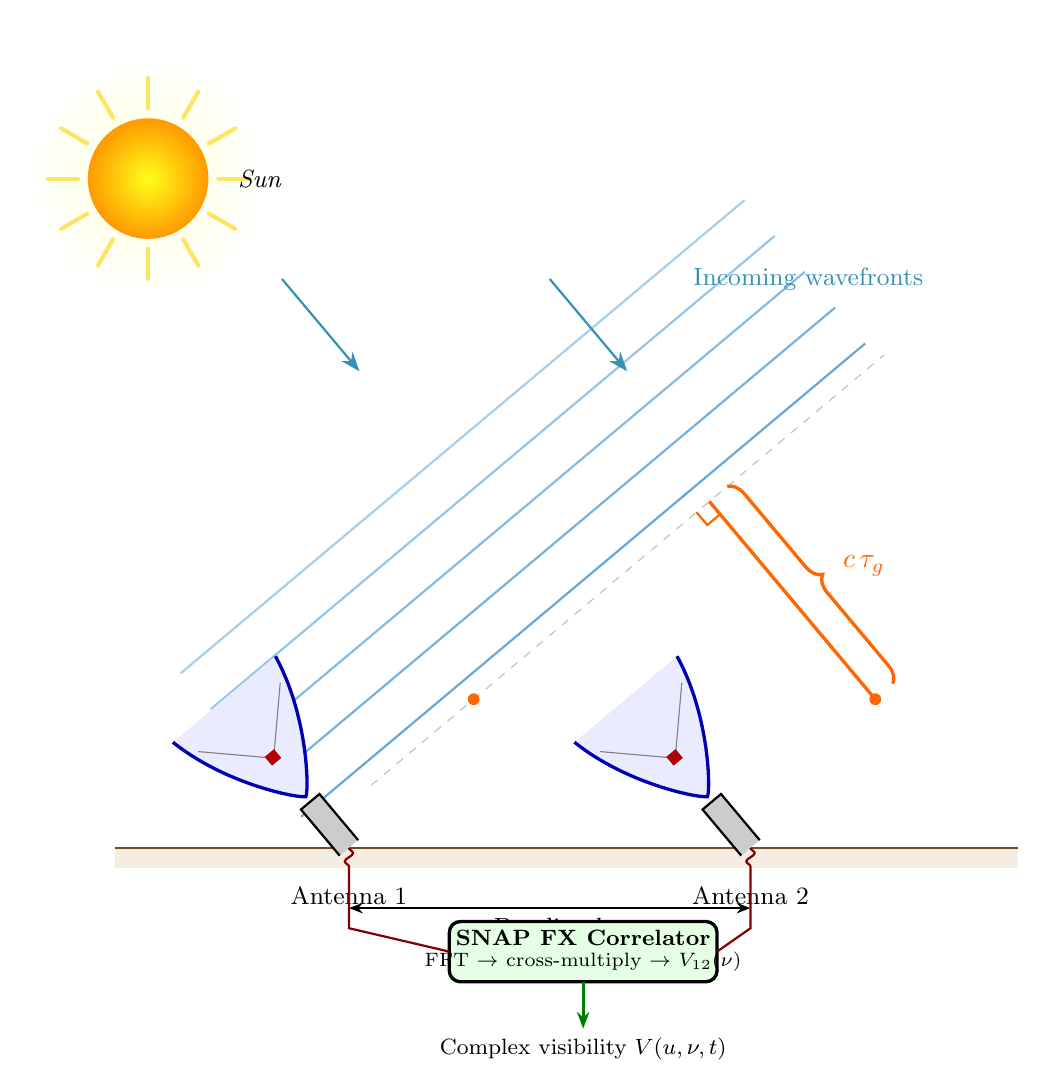
\begin{tikzpicture}[scale=0.85, every node/.style={font=\small}]
  %
  % Layout: Sun at upper-left, antennas at lower-right.
  % Source direction from antennas to Sun ~ 40 deg from vertical toward the left.
  % Dishes rotate 40 deg CCW so their apertures face the Sun.
  % Wavefronts are perpendicular to this direction and span both dishes.
  %
  % Source direction unit vector (toward Sun):
  %   s = (-sin40, cos40) = (-0.6428, 0.7660)
  % Wavefront direction (perpendicular to s):
  %   w = ( cos40, sin40) = ( 0.7660, 0.6428)
  %

  % === The Sun (upper-left) ===
  \shade[inner color=yellow!30, outer color=white, opacity=0.5] (-6.5,10.0) circle (1.8);
  \foreach \a in {0,30,...,330} {
    \draw[yellow!70!orange, line width=1.5pt, line cap=round, opacity=0.6]
      (-6.5,10.0) ++(\a:1.05) -- ++(\a:0.45);
  }
  \shade[inner color=yellow!90!white, outer color=orange!80!yellow] (-6.5,10.0) circle (0.9);
  \node[right] at (-5.3,10.0) {\textit{Sun}};

  % === Wavefronts ===
  % Place 5 wavefronts between the Sun and the dishes, spanning the full
  % width of both antennas. Centre each wavefront on the midpoint of the
  % two dishes (x=0, y~2.5) and shift successive fronts toward the Sun.
  \foreach \i in {0,1,2,3,4} {
    \pgfmathsetmacro{\dshift}{\i*0.7}  % shift toward Sun along s
    % Centre of this wavefront, offset along s from (0, 3.5):
    \pgfmathsetmacro{\cx}{0.0 + \dshift*(-0.6428)}
    \pgfmathsetmacro{\cy}{4.0 + \dshift*( 0.7660)}
    % Draw the wavefront line (direction w, length ±5.5 units)
    \draw[cyan!60!blue, thick, opacity={0.65-\i*0.07}]
      ({\cx - 5.5*0.7660}, {\cy - 5.5*0.6428})
      -- ({\cx + 5.5*0.7660}, {\cy + 5.5*0.6428});
  }

  % === Arrows showing incoming wave direction ===
  \draw[-{Stealth[length=7pt]}, thick, cyan!70!black]
    (-4.5,8.5) -- ({-4.5+1.8*0.6428}, {8.5-1.8*0.7660});
  \draw[-{Stealth[length=7pt]}, thick, cyan!70!black]
    (-0.5,8.5) -- ({-0.5+1.8*0.6428}, {8.5-1.8*0.7660});
  \node[cyan!70!black, right] at (1.5,8.5) {Incoming wavefronts};

  % === Ground ===
  \fill[brown!15] (-7.0,-0.3) rectangle (6.5,0);
  \draw[thick, brown!60!black] (-7.0,0) -- (6.5,0);

  % === Dish 1 (left), rotated 40 deg CCW ===
  \begin{scope}[shift={(-3.5,0)}, rotate=40]
    \fill[gray!40] (-0.18,0) rectangle (0.18,0.9);
    \draw[thick] (-0.18,0) -- (-0.18,0.9) -- (0.18,0.9) -- (0.18,0);
    \draw[very thick, blue!70!black, fill=blue!8]
      (-1.0,2.9) .. controls (-0.8,1.9) and (-0.1,1.05) .. (0,1.0)
      .. controls (0.1,1.05) and (0.8,1.9) .. (1.0,2.9);
    \draw[thin, gray] (-0.8,2.55) -- (0,1.75);
    \draw[thin, gray] (0.8,2.55) -- (0,1.75);
    \fill[red!70!black] (-0.09,1.68) rectangle (0.09,1.85);
  \end{scope}
  \draw[thick, red!50!black, decorate, decoration={snake, amplitude=1.5pt, segment length=6pt}]
    (-3.5,0.0) -- (-3.5,-0.3);
  \node[below] at (-3.5,-0.45) {Antenna 1};

  % === Dish 2 (right), rotated 40 deg CCW ===
  \begin{scope}[shift={(2.5,0)}, rotate=40]
    \fill[gray!40] (-0.18,0) rectangle (0.18,0.9);
    \draw[thick] (-0.18,0) -- (-0.18,0.9) -- (0.18,0.9) -- (0.18,0);
    \draw[very thick, blue!70!black, fill=blue!8]
      (-1.0,2.9) .. controls (-0.8,1.9) and (-0.1,1.05) .. (0,1.0)
      .. controls (0.1,1.05) and (0.8,1.9) .. (1.0,2.9);
    \draw[thin, gray] (-0.8,2.55) -- (0,1.75);
    \draw[thin, gray] (0.8,2.55) -- (0,1.75);
    \fill[red!70!black] (-0.09,1.68) rectangle (0.09,1.85);
  \end{scope}
  \draw[thick, red!50!black, decorate, decoration={snake, amplitude=1.5pt, segment length=6pt}]
    (2.5,0.0) -- (2.5,-0.3);
  \node[below] at (2.5,-0.45) {Antenna 2};

  % === Baseline annotation ===
  \draw[{Stealth[length=5pt]}-{Stealth[length=5pt]}, thick] (-3.5,-0.9) -- (2.5,-0.9);
  \node[below] at (-0.5,-0.9) {Baseline $b$};

  % === Geometric delay annotation ===
  % Dish tops (local (0,2.9) rotated 40 deg about base):
  %   dx = 2.9*sin40 = 1.864,  dy = 2.9*cos40 = 2.221
  %   D1top = (-2.0+1.864, 2.221) = (-0.136, 2.221)
  %   D2top = ( 4.0+1.864, 2.221) = ( 5.864, 2.221)
  %
  % Extra path for D2 = projection of baseline (D1->D2 = (6,0)) onto s:
  %   6 * (-0.6428) = -3.857
  % D2 is 3.857 units behind D1 along the source direction.
  %
  % Wavefront through D1top: pass through D1top along w.
  % Foot of perpendicular from D2top:
  %   component of (D2top-D1top)=(6,0) along w = 6*0.7660 = 4.596
  %   Foot = D1top + 4.596*w = (-0.136+3.521, 2.221+2.955) = (3.385, 5.176)

  \coordinate (D1top) at (-1.636, 2.221);
  \coordinate (D2top) at (4.364, 2.221);
  \coordinate (D2foot) at (1.885, 5.176);

  % Wavefront reference line through D1top
  \draw[thin, dashed, gray!50]
    ($(D1top) + (-2.0*0.7660, -2.0*0.6428)$) -- ($(D1top) + (8.0*0.7660, 8.0*0.6428)$);

  % Extra path line from D2top to D2foot
  \draw[very thick, orange!80!red] (D2top) -- (D2foot);

  % Right-angle marker at D2foot
  \coordinate (rA) at ($(D2foot) + (-0.25*0.7660, -0.25*0.6428)$);
  \coordinate (rC) at ($(D2foot) + (0.25*0.6428, -0.25*0.7660)$);
  \coordinate (rB) at ($(rA) + (0.25*0.6428, -0.25*0.7660)$);
  \draw[orange!80!red, thick] (rA) -- (rB) -- (rC);

  % Brace along the extra path, offset outward (along +w direction)
  \draw[very thick, orange!80!red, decorate, decoration={brace, amplitude=6pt}]
    ($(D2foot) + (0.35*0.7660, 0.35*0.6428)$) -- ($(D2top) + (0.35*0.7660, 0.35*0.6428)$);
  \node[right, orange!80!red, font=\normalsize\bfseries]
    at ($(D2top)!0.5!(D2foot) + (0.8*0.7660, 0.8*0.6428)$) {$c\,\tau_g$};

  % Dots at dish tops
  \fill[orange!80!red] (D1top) circle (2.5pt);
  \fill[orange!80!red] (D2top) circle (2.5pt);

  % === SNAP correlator box ===
  \draw[very thick, fill=green!10, rounded corners=4pt]
    (-2.0,-2.0) rectangle (2.0,-1.1);
  \node[font=\footnotesize\bfseries] at (0,-1.35) {SNAP FX Correlator};
  \node[font=\scriptsize] at (0,-1.7) {FFT $\rightarrow$ cross-multiply $\rightarrow$ $V_{12}(\nu)$};

  % Cables from dishes to correlator
  \draw[thick, red!50!black] (-3.5,-0.3) -- (-3.5,-1.2) -- (-2.0,-1.55);
  \draw[thick, red!50!black] (2.5,-0.3) -- (2.5,-1.2) -- (2.0,-1.55);

  % Output arrow
  \draw[-{Stealth[length=6pt]}, very thick, green!50!black]
    (0,-2.0) -- (0,-2.7);
  \node[below, font=\footnotesize] at (0,-2.7) {Complex visibility $V(u, \nu, t)$};

\end{tikzpicture}
\caption{Schematic of the two-dish correlating interferometer. Two dishes separated by baseline $b$ observe an extended source (the Sun). Plane wavefronts arrive at the two antennas with a relative geometric delay $\tau_g = b\cos\delta\,\sin h / c$, which depends on the projected baseline perpendicular to the source direction. The signals are brought together in the SNAP FX correlator, which digitises, Fourier-transforms, and cross-multiplies the voltages to produce the complex visibility spectrum $V_{12}(\nu, t)$. As the Earth rotates, $\tau_g$ changes, and the correlated output traces out the interferometric fringe.}
\label{fig:interferometer}
\end{figure*}


\begin{figure}[H]
\centering
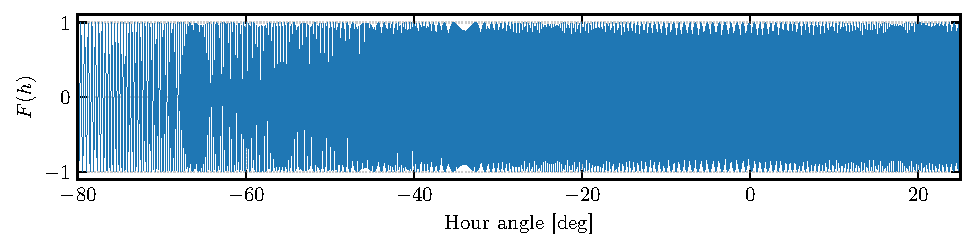
\includegraphics[width=\columnwidth]{figures/fig_fringe_synthetic.pdf}
\caption{Synthetic point-source fringe pattern $F(h)$ versus hour angle for our interferometer parameters ($b_{\mathrm{ew}} = 15.17$~m, $\nu = 10.45$~GHz, $\delta \approx 0^\circ$). The fringe frequency increases toward transit ($h = 0$) as the projected baseline grows. For the Sun, the amplitude of this pattern is modulated by the Bessel-function visibility envelope (\S\ref{sec:jinc}).}
\label{fig:fringe_synthetic}
\end{figure}

\subsection{The Adding Interferometer and Path Delay}
\label{sec:delay}

Consider two antennas separated by a baseline vector $\mathbf{b}$ observing a distant source at hour angle $h$ and declination $\delta$, from a site at terrestrial latitude $L$. The signals arrive at the two antennas with a relative path delay that depends on the projected baseline perpendicular to the line of sight. We decompose the baseline into an east--west component $b_{\mathrm{ew}}$ and a north--south component $b_{\mathrm{ns}}$, following the standard two-dish formalism \citep{TMS2017, FomalontWright1974}.

The east--west baseline contributes a geometric delay
\begin{equation}
\label{eq:delay_ew}
\tau_{g,\mathrm{ew}}(h) = \frac{b_{\mathrm{ew}}}{c}\cos\delta\,\sin h,
\end{equation}
and the north--south baseline contributes
\begin{equation}
\label{eq:delay_ns}
\tau_{g,\mathrm{ns}}(h) = \frac{b_{\mathrm{ns}}}{c}\sin L\,\cos\delta\,\cos h
  - \frac{b_{\mathrm{ns}}}{c}\cos L\,\sin\delta.
\end{equation}
The first term of \eqref{eq:delay_ns} varies with hour angle (the projection perpendicular to the Earth's rotation axis), while the second is constant in $h$. Since it is independent of $h$, we absorb this constant NS term into the instrumental cable delay $\tau_c$, defining an effective geometric delay
\begin{equation}
\label{eq:delay_combined}
\tau'_g(h) = \frac{b_{\mathrm{ew}}}{c}\cos\delta\,\sin h
  + \frac{b_{\mathrm{ns}}}{c}\sin L\,\cos\delta\,\cos h
\end{equation}
and a modified cable delay
\begin{equation}
\label{eq:tauc_prime}
\tau'_c = \tau_c - \frac{b_{\mathrm{ns}}}{c}\cos L\,\sin\delta.
\end{equation}
The total relative delay between the two signal paths is $\tau_{\mathrm{tot}} = \tau'_g(h) + \tau'_c$.


\subsection{The Point-Source Fringe}
\label{sec:fringe}

The NCH interferometer is a \emph{correlating} interferometer: the SNAP FX correlator independently digitises and Fourier-transforms the voltage from each antenna, then cross-multiplies the complex spectra to produce the visibility $V_{12}(\nu) = \langle \tilde{v}_1(\nu)\,\tilde{v}_2^*(\nu)\rangle$ \citep{TMS2017}. This is equivalent to measuring the cross-correlation of the two signals at the relative delay $\tau_{\mathrm{tot}}$, and yields the fringe directly without the total-power (DC) terms that appear in an adding interferometer \citep{Ryle1952}. In practice, residual DC offsets from instrumental effects still contaminate the real part of the visibility and must be removed (\S\ref{sec:dc}).

To derive the fringe equation, consider a monochromatic point source of frequency $\nu$. The voltages are
\begin{align}
E_1(t) &= \cos(2\pi\nu t), \label{eq:E1} \\
E_2(t) &= \cos\!\bigl(2\pi\nu\,[t + \tau_{\mathrm{tot}}]\bigr). \label{eq:E2}
\end{align}
The correlator output is proportional to $\langle E_1(t)\,E_2(t)\rangle$, the time-averaged product of the two signals. Using the identity $\cos A\cos B = \tfrac{1}{2}[\cos(A-B) + \cos(A+B)]$ and noting that the sum-frequency term averages to zero, the fringe output is
\begin{equation}
\label{eq:fringe_product}
F(h) = \cos\!\bigl(2\pi\nu\,[\tau'_g(h) + \tau'_c]\bigr).
\end{equation}
Applying the angle-addition identity $\cos(\alpha + \beta) = \cos\alpha\cos\beta - \sin\alpha\sin\beta$, we write this in the standard least-squares form:
\begin{equation}
\label{eq:fringe_boxed}
F(h) = A\cos\!\bigl(2\pi\nu\,\tau'_g\bigr) + B\sin\!\bigl(2\pi\nu\,\tau'_g\bigr),
\end{equation}
where $A = \cos(2\pi\nu\,\tau'_c)$ and $B = -\sin(2\pi\nu\,\tau'_c)$ are unknown constants that encode the instrumental phase. Crucially, the unknown baseline parameters appear \emph{only} inside $\tau'_g$; the constants $A$ and $B$ are linear and can be solved analytically by standard least squares for any trial value of the baseline, making this a separable nonlinear least-squares problem \citep{Golub1973}.

\paragraph{Three physical interpretations of the fringe.}
The fringe admits three complementary physical pictures:
\begin{enumerate}
\item \emph{Giant sine wave in the sky.} The interferometer projects a sinusoidal sensitivity pattern onto the sky with fringe spacing $\lambda/b_{\mathrm{proj}}$ radians, where $b_{\mathrm{proj}}$ is the projected baseline perpendicular to the line of sight. As the Earth rotates, a point source drifts through alternating positive and negative lobes, and the output oscillates. For an extended source, the output depends on how the source fills the fringes---when the fringe spacing matches the source diameter, positive and negative lobes cancel and the response goes to zero.

\item \emph{Giant DSB mixer.} The fringe operates like a double-sideband mixer: the two antennas ``beat'' the sky signal against each other at the geometric delay rate, down-converting the spatial brightness distribution into a temporal fringe that can be sampled and recorded.

\item \emph{Correlation function.} The complex visibility $V_{12}(\tau) = \langle E_1(t)\,E_2^*(t+\tau)\rangle$ is the mutual coherence function of the electric field at the two antenna locations. By the van~Cittert--Zernike theorem (\S\ref{sec:vCZ}), this is the Fourier transform of the sky brightness distribution \citep{vanCittert1934, Zernike1938, TMS2017}.
\end{enumerate}


Figure~\ref{fig:fringe_on_sky} illustrates the ``sine wave in the sky'' picture for an extended source. At large hour angles (left panel), the projected baseline is short, the fringes are wide, and the solar disk fits within a single positive lobe---the visibility is high. Near transit (right panel), the projected baseline is long, the fringes are narrow, and the disk spans multiple lobes whose positive and negative contributions partially cancel---the visibility drops. At a Bessel null, the cancellation is exact and the visibility vanishes.

\begin{figure*}[t]
\centering
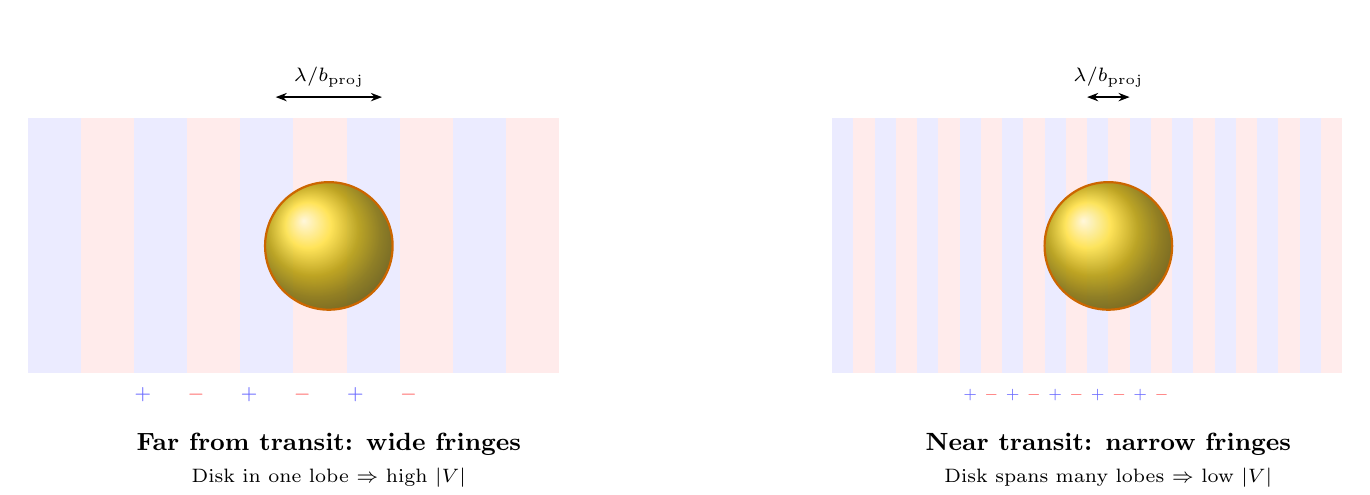
\begin{tikzpicture}[scale=0.9, every node/.style={font=\small}]

  % === Panel 1: Far from transit (wide fringes, high visibility) ===
  \begin{scope}[shift={(-5.5,0)}]
    % Fringes (wide spacing)
    \foreach \x in {-3.5,-2.0,...,3.5} {
      \fill[blue!8] (\x-0.75, -1.8) rectangle (\x, 1.8);
      \fill[red!8]  (\x, -1.8) rectangle (\x+0.75, 1.8);
    }
    % Fringe labels
    \node[font=\scriptsize, blue!60] at (-2.625, -2.1) {$+$};
    \node[font=\scriptsize, red!60] at (-1.875, -2.1) {$-$};
    \node[font=\scriptsize, blue!60] at (-1.125, -2.1) {$+$};
    \node[font=\scriptsize, red!60] at (-0.375, -2.1) {$-$};
    \node[font=\scriptsize, blue!60] at (0.375, -2.1) {$+$};
    \node[font=\scriptsize, red!60] at (1.125, -2.1) {$-$};

    % Solar disk
    \shade[ball color=yellow!70!orange, opacity=0.85] (0,0) circle (0.9);
    \draw[thick, orange!80!black] (0,0) circle (0.9);

    % Fringe spacing annotation
    \draw[{Stealth[length=4pt]}-{Stealth[length=4pt]}, thick]
      (-0.75, 2.1) -- (0.75, 2.1);
    \node[above, font=\scriptsize] at (0, 2.1) {$\lambda/b_{\mathrm{proj}}$};

    % Title
    \node[font=\small\bfseries, below] at (0, -2.5)
      {Far from transit: wide fringes};
    \node[font=\scriptsize, below] at (0, -3.0)
      {Disk in one lobe $\Rightarrow$ high $|V|$};
  \end{scope}

  % === Panel 2: Near transit (narrow fringes, low visibility) ===
  \begin{scope}[shift={(5.5,0)}]
    % Fringes (narrow spacing)
    \foreach \x in {-3.6,-3.0,...,3.6} {
      \fill[blue!8] (\x-0.3, -1.8) rectangle (\x, 1.8);
      \fill[red!8]  (\x, -1.8) rectangle (\x+0.3, 1.8);
    }
    % Fringe labels
    \node[font=\tiny, blue!60] at (-1.95, -2.1) {$+$};
    \node[font=\tiny, red!60] at (-1.65, -2.1) {$-$};
    \node[font=\tiny, blue!60] at (-1.35, -2.1) {$+$};
    \node[font=\tiny, red!60] at (-1.05, -2.1) {$-$};
    \node[font=\tiny, blue!60] at (-0.75, -2.1) {$+$};
    \node[font=\tiny, red!60] at (-0.45, -2.1) {$-$};
    \node[font=\tiny, blue!60] at (-0.15, -2.1) {$+$};
    \node[font=\tiny, red!60] at (0.15, -2.1) {$-$};
    \node[font=\tiny, blue!60] at (0.45, -2.1) {$+$};
    \node[font=\tiny, red!60] at (0.75, -2.1) {$-$};

    % Solar disk
    \shade[ball color=yellow!70!orange, opacity=0.85] (0,0) circle (0.9);
    \draw[thick, orange!80!black] (0,0) circle (0.9);

    % Fringe spacing annotation
    \draw[{Stealth[length=4pt]}-{Stealth[length=4pt]}, thick]
      (-0.3, 2.1) -- (0.3, 2.1);
    \node[above, font=\scriptsize] at (0, 2.1) {$\lambda/b_{\mathrm{proj}}$};

    % Title
    \node[font=\small\bfseries, below] at (0, -2.5)
      {Near transit: narrow fringes};
    \node[font=\scriptsize, below] at (0, -3.0)
      {Disk spans many lobes $\Rightarrow$ low $|V|$};
  \end{scope}

\end{tikzpicture}
\caption{The fringe pattern projected on the sky for an extended source (the Sun). \textit{Left:} Far from transit, the projected baseline is short and the fringe spacing $\lambda/b_{\mathrm{proj}}$ is wide; the solar disk fits within a single positive lobe, so the net response (visibility) is high. \textit{Right:} Near transit, the projected baseline is long and the fringes are narrow; the disk spans multiple positive ($+$) and negative ($-$) lobes whose contributions partially cancel, reducing the visibility. At a Bessel null, the cancellation is exact.}
\label{fig:fringe_on_sky}
\end{figure*}


\subsection{The Local Fringe Frequency}
\label{sec:fringefreq}

The fringe phase $\phi(h) = 2\pi\nu\,\tau'_g(h)$ varies with hour angle. The instantaneous fringe frequency is obtained by Taylor-expanding $\sin h$ and $\cos h$ about the current hour angle $h_0$ and retaining the first-order term in $\Delta h = h - h_0$. The result is
\begin{equation}
\label{eq:fringe_freq}
f_f(h) = \omega_\oplus\left[\frac{b_{\mathrm{ew}}}{\lambda}\cos\delta\,\cos h
  - \frac{b_{\mathrm{ns}}}{\lambda}\sin L\,\cos\delta\,\sin h\right],
\end{equation}
where $\omega_\oplus = 2\pi/(86164.09~\mathrm{s}) = 7.2921 \times 10^{-5}$~rad~s$^{-1}$ is the sidereal rotation rate \citep{TMS2017}. For our nearly east--west baseline ($b_{\mathrm{ew}} \approx 15$~m, $b_{\mathrm{ns}} \approx 1.5$~m) at $\lambda = 2.87$~cm and $\delta \approx 0^\circ$, the fringe frequency at the meridian ($h = 0$) is $f_f \approx 38$~mHz, corresponding to a fringe period of $\sim$26~s. This is the quantity we measure from Fourier analysis of the visibility time series and use to determine the baseline.

A subtlety: the hour angle tracks \emph{sidereal} time, not solar time. The sidereal day is 86164.09~s, versus the solar day of 86400~s---a 0.27\% difference. Over a full-track observation spanning $\sim$100$^\circ$ in hour angle, this corresponds to $\sim$4~cm of baseline shift if the wrong rate is used, which exceeds our formal fitting uncertainty.


\subsection{Fourier Analysis of the Fringe}
\label{sec:fourier_fringe}

The fringe signal in \eqref{eq:fringe_boxed} is a quasi-sinusoidal function of time whose instantaneous frequency $f_f(h)$ varies slowly as the Earth rotates. Several useful operations follow from this structure:

\begin{itemize}
\item \textbf{Power spectrum.} A Fourier transform of the visibility time series reveals a peak at the fringe frequency, providing an immediate sanity check that the fringes are real and the system is functioning. The peak should lie within the range of $f_f(h)$ predicted by \eqref{eq:fringe_freq} for the hour-angle coverage of the observation.
\item \textbf{Band-pass filtering.} The fringe signal occupies a narrow band around $f_f$, while the DC offset from total power and broadband noise are spectrally separated. A band-pass filter centred on the predicted fringe frequency isolates the fringe from these contaminants.
\item \textbf{Short-time Fourier transform (STFT).} By computing the FFT of overlapping windowed segments of the time series, we track the time-varying $f_f(h)$ as a function of hour angle \citep{Harris1978}. Fitting the measured $f_f(h)$ curve to \eqref{eq:fringe_freq} yields an independent baseline estimate (Method~1 in \S\ref{sec:baseline}).
\end{itemize}


\subsection{Extended Sources and the Van Cittert--Zernike Theorem}
\label{sec:vCZ}

For a point source, the interferometer output is the fringe pattern $F(h)$. For an extended source with one-dimensional intensity distribution $I(\Delta h)$ (where $\Delta h = h - h_s$ is the angular offset from the source centre $h_s$), the output is the integral of the point-source fringe weighted by the brightness distribution \citep{TMS2017}:
\begin{equation}
\label{eq:extended_integral}
R(h_s) = \int I(\Delta h)\,F(h_s + \Delta h)\,\mathrm{d}\Delta h.
\end{equation}
For a symmetric source ($I(\Delta h) = I(-\Delta h)$), the antisymmetric (sine) terms integrate to zero, and the response factors into two parts:
\begin{equation}
\label{eq:fringe_modulator}
R(h_s) = \underbrace{F(h_s)}_{\text{Point-source fringe}}
  \times
  \underbrace{\int I(\Delta h)\,\cos(2\pi f_f\,\Delta h)\,\mathrm{d}\Delta h}_{\text{Fringe modulator}}.
\end{equation}
The second factor---the \emph{fringe modulator} or \emph{modulating function}---is the cosine Fourier transform of the source brightness distribution, evaluated at the spatial frequency $f_f$ (cycles per radian on the sky). This is a statement of the van~Cittert--Zernike theorem \citep{vanCittert1934, Zernike1938}: \emph{the visibility measured by an interferometer is the Fourier transform of the sky brightness distribution}. The zeros of the modulating function occur when the fringe spacing matches the source size so that equal areas of the source fall on positive and negative fringe lobes, and the net response cancels.


\subsection{Uniform Disk Visibility: The Bessel/Jinc Function}
\label{sec:jinc}

We model the Sun as a uniformly bright circular disk of angular radius $R$. The one-dimensional projection of this disk at angular offset $\theta$ from centre is
\begin{equation}
\label{eq:disk_profile}
I(\theta) = \frac{2}{\pi R^2}\sqrt{R^2 - \theta^2},\quad |\theta| < R,
\end{equation}
normalised so that $\int_{-R}^{R}I(\theta)\,\mathrm{d}\theta = 1$. Substituting into the modulating function integral (\eqref{eq:fringe_modulator}) and using the change of variables $\theta = R\cos\vartheta$ yields the analytic result \citep{BornWolf1999}:
\begin{equation}
\label{eq:jinc}
\frac{V(|u|)}{V(0)} = \frac{2\,J_1(2\pi\,|u|\,R)}{2\pi\,|u|\,R},
\end{equation}
where $|u| = |u_{\mathrm{sky}}|$ is the projected baseline in wavelengths and $J_1$ is the Bessel function of the first kind of order one. This function, often called the ``jinc'' function, has zero crossings at the projected baselines $|u|\,R = j_{1,k}/(2\pi)$, where $j_{1,k}$ are the zeros of $J_1$ ($j_{1,1} = 3.832$, $j_{1,2} = 7.016$, $j_{1,3} = 10.174$, $j_{1,4} = 13.324$; \citealt{AS1965}).

The lab manual also prescribes a \emph{discrete-sum} form of the modulating function, in which the integral is replaced by a Riemann sum over $2N+1$ slices:
\begin{equation}
\label{eq:mf_discrete}
\mathrm{MF}_{\mathrm{theory}} \approx \delta h \sum_{n=-N}^{+N}
\left[1 - \left(\frac{n}{N}\right)^2\right]^{1/2}
\cos\!\left(\frac{2\pi f_f R\,n}{N}\right).
\end{equation}
We verify numerically (\S\ref{sec:jinc_fit}) that this discrete-sum form converges to the analytic jinc to better than $10^{-4}$ for $N \geq 100$, confirming that the zero-crossing positions are identical. Figure~\ref{fig:bessel_theory} shows the jinc function with the first four Bessel zeros marked.

\begin{figure}[H]
\centering
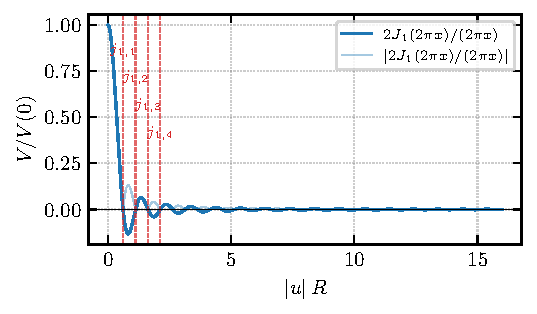
\includegraphics[width=\columnwidth]{figures/fig_bessel_envelope_theory.pdf}
\caption{Theoretical visibility amplitude for a uniform circular disk as a function of the dimensionless baseline $|u|\,R$. The solid line shows the signed jinc function $2J_1(2\pi|u|R)/(2\pi|u|R)$; the lighter line shows its absolute value. Vertical dashed lines mark the first four Bessel zeros $j_{1,k}/(2\pi)$, at which the visibility crosses zero and the fringe vanishes.}
\label{fig:bessel_theory}
\end{figure}


\subsection{Measuring the Solar Diameter}
\label{sec:diameter_theory}

The zero crossings of the jinc function provide a direct measurement of the solar radius. At the $k$-th null, the projected baseline satisfies $|u_k|\,R = j_{1,k}/(2\pi)$, so
\begin{equation}
\label{eq:diameter_from_null}
R = \frac{j_{1,k}}{2\pi\,|u_k|}.
\end{equation}
Each observed null yields an independent radius estimate; the mean over all matched nulls gives the adopted value. Equivalently, one can fit the jinc function to the observed fringe-amplitude envelope with $R$ as a free parameter.

\paragraph{Limb-brightened disk.}
At centimetre wavelengths, the solar brightness distribution is not uniform: the limb is brighter than the disk centre because the line of sight at the limb passes through more of the chromospheric temperature inversion \citep{Stix2002, Dulk1985}. We generalise the uniform-disk model by adding a quadratic limb-brightening term:
\begin{equation}
\label{eq:limb_bright}
V_{\mathrm{lb}}(q) = \frac{\displaystyle\frac{2\,J_1(x)}{x} + \varepsilon\cdot 2\!\int_0^1 t^3\,J_0(x\,t)\,\mathrm{d}t}{1 + \varepsilon/2},
\end{equation}
where $x = 2\pi\,q\,R$ and $\varepsilon$ parameterises the degree of limb brightening. When $\varepsilon = 0$, this reduces to the jinc. The denominator ensures $V_{\mathrm{lb}}(0) = 1$.

\paragraph{Sunspot floor.}
An unresolved active region at angular offset $(\Delta\alpha, \Delta\delta)$ from disk centre contributes a point-source component that adds in quadrature to the disk visibility, producing a non-zero floor at the Bessel nulls. The combined model is
\begin{equation}
\label{eq:sunspot_model}
|V(q)| = A\,\sqrt{V_{\mathrm{lb}}(q;\,R,\,\varepsilon)^2 + f^2},
\end{equation}
where $f$ is the sunspot flux fraction (the fraction of the total flux contributed by the unresolved source) and $A$ is an overall amplitude. The amplitude at the Bessel nulls is then $A\,f$, directly measuring the spot flux.


%%% ---------------------------------------------------------------
\section{Instrument and Observations}
\label{sec:obs}
%%% ---------------------------------------------------------------

\subsection{The X-Band Interferometer}
\label{sec:instrument}

The NCH interferometer consists of two dishes on the roof of Campbell Hall, with a nearly east--west baseline. Each dish feeds a double-conversion heterodyne receiver: the first local oscillator (LO1 at 8.75~GHz) converts the sky signal from the RF band ($\sim$10.45~GHz) to an intermediate frequency (IF), and the second local oscillator (LO2 at 1.54~GHz) down-converts the IF to baseband for sampling. An FX correlator implemented on a SNAP signal-processing board digitises both signals at 500~Msps, computes a 2048-point real FFT (yielding 1024 spectral channels with channel spacing $\Delta\nu = F_s/N_{\mathrm{FFT}} = 244$~kHz), and cross-multiplies the resulting complex voltage spectra. The cross-correlation is integrated over 305,200 spectra, corresponding to an integration time of 1.25~s per visibility. Table~\ref{tab:system} summarises the key system parameters.

\begin{table}[H]
\centering
\caption{System parameters of the NCH X-band interferometer.}
\label{tab:system}
\begin{tabular}{lc}
\toprule
Parameter & Value \\
\midrule
LO1 frequency & 8.750~GHz \\
LO2 frequency & 1.540~GHz \\
Sky frequency (band centre) & 10.450~GHz \\
Total bandwidth & 250~MHz \\
Analysis band & 10.415--10.485~GHz \\
Sample rate ($F_s$) & 500~Msps \\
FFT length ($N_{\mathrm{FFT}}$) & 2048 \\
Output channels & 1024 \\
Channel spacing ($\Delta\nu$) & 244~kHz \\
Integration time & 1.25~s \\
Observatory latitude ($L$) & $37.8732^\circ$~N \\
Observatory longitude & $122.2571^\circ$~W \\
\bottomrule
\end{tabular}
\end{table}

Figure~\ref{fig:signal_path} shows a summary block diagram of the signal path for one antenna; the full detailed diagram is reproduced in Appendix~\ref{app:signal_path}. Each antenna signal undergoes two frequency conversions: a DSB mixer with LO1 (8.75~GHz) converts the X-band RF to an IF near 1.7~GHz, and an SSB mixer with LO2 (1.54~GHz, Valon synthesiser) converts the IF to baseband for digitisation by the SNAP board.

\begin{figure*}[t]
\centering
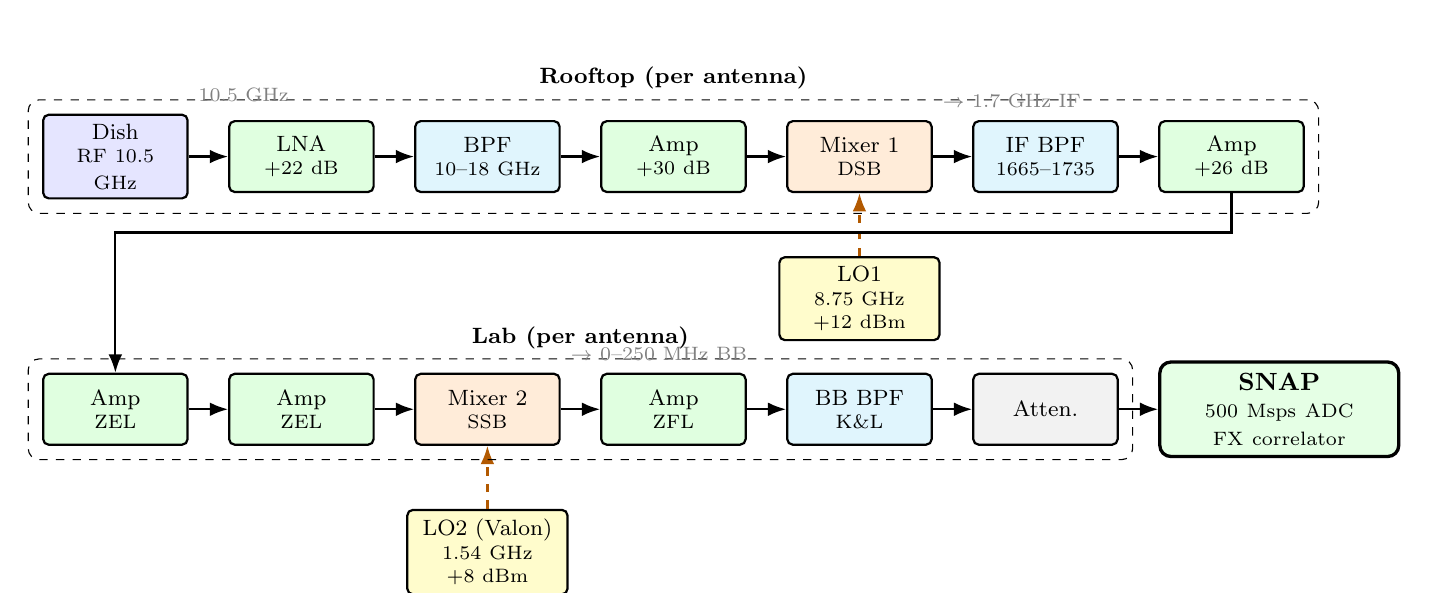
\begin{tikzpicture}[
    rfbox/.style={draw, thick, rounded corners=2pt, align=center,
                  font=\footnotesize, minimum height=0.9cm, text width=1.6cm},
    ampbox/.style={rfbox, fill=green!12},
    filtbox/.style={rfbox, fill=cyan!12},
    mixbox/.style={rfbox, fill=orange!15},
    lobox/.style={rfbox, fill=yellow!20, text width=1.8cm},
    snapbox/.style={draw, very thick, rounded corners=4pt, fill=green!10,
                    align=center, font=\small, text width=2.8cm, minimum height=1.2cm},
    chainarrow/.style={-Latex, thick},
    loarrow/.style={-Latex, thick, dashed, orange!70!black},
    sectionbox/.style={draw, dashed, rounded corners, inner sep=5pt,
                       label={[font=\footnotesize\bfseries]above:#1}},
  ]

  % === Row: Rooftop chain (one antenna) ===
  \node[rfbox, fill=blue!10] (ant) at (0,0) {Dish\\[-1pt]{\scriptsize RF 10.5 GHz}};
  \node[ampbox, right=5mm of ant] (lna) {LNA\\[-1pt]{\scriptsize +22 dB}};
  \node[filtbox, right=5mm of lna] (bpf1) {BPF\\[-1pt]{\scriptsize 10--18 GHz}};
  \node[ampbox, right=5mm of bpf1] (amp1) {Amp\\[-1pt]{\scriptsize +30 dB}};
  \node[mixbox, right=5mm of amp1] (mix1) {Mixer 1\\[-1pt]{\scriptsize DSB}};
  \node[filtbox, right=5mm of mix1] (bpf2) {IF BPF\\[-1pt]{\scriptsize 1665--1735}};
  \node[ampbox, right=5mm of bpf2] (amp2) {Amp\\[-1pt]{\scriptsize +26 dB}};

  % Arrows
  \draw[chainarrow] (ant) -- (lna);
  \draw[chainarrow] (lna) -- (bpf1);
  \draw[chainarrow] (bpf1) -- (amp1);
  \draw[chainarrow] (amp1) -- (mix1);
  \draw[chainarrow] (mix1) -- (bpf2);
  \draw[chainarrow] (bpf2) -- (amp2);

  % LO1
  \node[lobox, below=8mm of mix1] (lo1) {LO1\\[-1pt]{\scriptsize 8.75 GHz}\\[-1pt]{\scriptsize +12 dBm}};
  \draw[loarrow] (lo1) -- (mix1);

  % Section box
  \node[sectionbox={Rooftop (per antenna)},
        fit=(ant)(lna)(bpf1)(amp1)(mix1)(bpf2)(amp2)] {};

  % === Row: Lab chain ===
  \node[ampbox, below=22mm of ant] (lab1) {Amp\\[-1pt]{\scriptsize ZEL}};
  \node[ampbox, right=5mm of lab1] (lab2) {Amp\\[-1pt]{\scriptsize ZEL}};
  \node[mixbox, right=5mm of lab2] (mix2) {Mixer 2\\[-1pt]{\scriptsize SSB}};
  \node[ampbox, right=5mm of mix2] (lab3) {Amp\\[-1pt]{\scriptsize ZFL}};
  \node[filtbox, right=5mm of lab3] (bpf3) {BB BPF\\[-1pt]{\scriptsize K\&L}};
  \node[rfbox, fill=gray!10, right=5mm of bpf3] (atten) {Atten.};

  % SNAP
  \node[snapbox, right=5mm of atten] (snap) {\textbf{SNAP}\\[-1pt]{\scriptsize 500 Msps ADC}\\[-1pt]{\scriptsize FX correlator}};

  % Lab arrows
  \draw[chainarrow] (amp2.south) -- ++(0,-5mm) -| (lab1.north);
  \draw[chainarrow] (lab1) -- (lab2);
  \draw[chainarrow] (lab2) -- (mix2);
  \draw[chainarrow] (mix2) -- (lab3);
  \draw[chainarrow] (lab3) -- (bpf3);
  \draw[chainarrow] (bpf3) -- (atten);
  \draw[chainarrow] (atten) -- (snap);

  % LO2
  \node[lobox, below=8mm of mix2] (lo2) {LO2 (Valon)\\[-1pt]{\scriptsize 1.54 GHz}\\[-1pt]{\scriptsize +8 dBm}};
  \draw[loarrow] (lo2) -- (mix2);

  % Section box
  \node[sectionbox={Lab (per antenna)},
        fit=(lab1)(lab2)(mix2)(lab3)(bpf3)(atten)] {};

  % Frequency annotations
  \node[font=\scriptsize, gray, above=1pt of ant.north east, anchor=south west] {10.5 GHz};
  \node[font=\scriptsize, gray, above=1pt of mix1.north east, anchor=south west] {$\to$ 1.7 GHz IF};
  \node[font=\scriptsize, gray, above=1pt of mix2.north east, anchor=south west] {$\to$ 0--250 MHz BB};

\end{tikzpicture}
\caption{Summary signal path for one antenna of the NCH interferometer. The X-band RF signal ($\sim$10.5~GHz) is amplified, filtered, and down-converted to IF ($\sim$1.7~GHz) by DSB Mixer~1 with LO1 at 8.75~GHz. In the lab, SSB Mixer~2 with LO2 at 1.54~GHz converts to baseband (0--250~MHz) for digitisation by the SNAP FX correlator. Both antennas share the same LO1 and LO2 sources. The full detailed signal diagram is reproduced in Appendix~\ref{app:signal_path}.}
\label{fig:signal_path}
\end{figure*}


\subsection{Observations}
\label{sec:observations}

Horizon-to-horizon drift-scan observations of the Sun were obtained on 2026 March~20 (UTC). The data span hour angles from $-79.9^\circ$ to $+22.0^\circ$, totalling 8226 visibility integrations divided across three observation ``chips'' (contiguous runs separated by brief instrumental interruptions). The Sun's declination during the observation was $\delta \approx -0.083^\circ$. Table~\ref{tab:obslog} summarises the observation log.

\begin{table}[H]
\centering
\caption{Observation log. Each ``chip'' is a contiguous run of captures separated by brief gaps.}
\label{tab:obslog}
\begin{tabular}{cccc}
\toprule
Chip & Captures & HA range [deg] & Duration [hr] \\
\midrule
0 & 5514 & $-79.9$ to $-8.0$ & 4.8 \\
1 & 403 & $-7.7$ to $-5.3$ & 0.2 \\
2 & 2309 & $-3.3$ to $+22.0$ & 1.7 \\
\bottomrule
\end{tabular}
\end{table}


\subsection{Instrument Calibration}
\label{sec:calibration}

An independent baseline survey was performed using the LiDAR sensor of an iPhone~13~Pro, yielding $b_{\mathrm{ew}}^{\mathrm{lidar}} = 15.17 \pm 0.30$~m and $b_{\mathrm{ns}}^{\mathrm{lidar}} = 1.36 \pm 0.30$~m. The conservative 30~cm uncertainty encompasses both the single-shot ranging accuracy at $\sim$15~m distance and the difficulty of identifying the antenna phase centre by eye.

Channels at multiples of 256 (indices 0, 256, 512, 768) are contaminated by DC and FPGA pipeline harmonics and are excluded from all analysis. The usable analysis band is restricted to 10.415--10.485~GHz (70~MHz), where the IF bandpass is flattest, yielding 285 good channels.

Per-chip gain ratios are measured from the median $|V|$ in the analysis band, relative to Chip~0. Chip~2 shows a $\sim$10\% excess gain, consistent with a back-end attenuator change or LNA drift. This gain step is corrected before envelope fitting in \S\ref{sec:diameter}.


%%% ---------------------------------------------------------------
\section{Data Reduction}
\label{sec:reduction}
%%% ---------------------------------------------------------------

\subsection{Raw Data Inspection}
\label{sec:raw}

Figure~\ref{fig:raw_vis} shows the raw complex visibility at a representative mid-band channel (ch~655, 10.450~GHz) as a function of hour angle. The real part exhibits a slowly varying DC pedestal superimposed on the oscillating fringe, while the imaginary part oscillates about zero. The fringe frequency decreases away from the meridian, consistent with the $\cos h$ dependence in \eqref{eq:fringe_freq}. Figure~\ref{fig:amp_spectrum} shows the time-averaged amplitude spectrum across the full 250~MHz Nyquist band, illustrating the IF bandpass shape and the location of the analysis band.

\begin{figure*}[t]
\centering
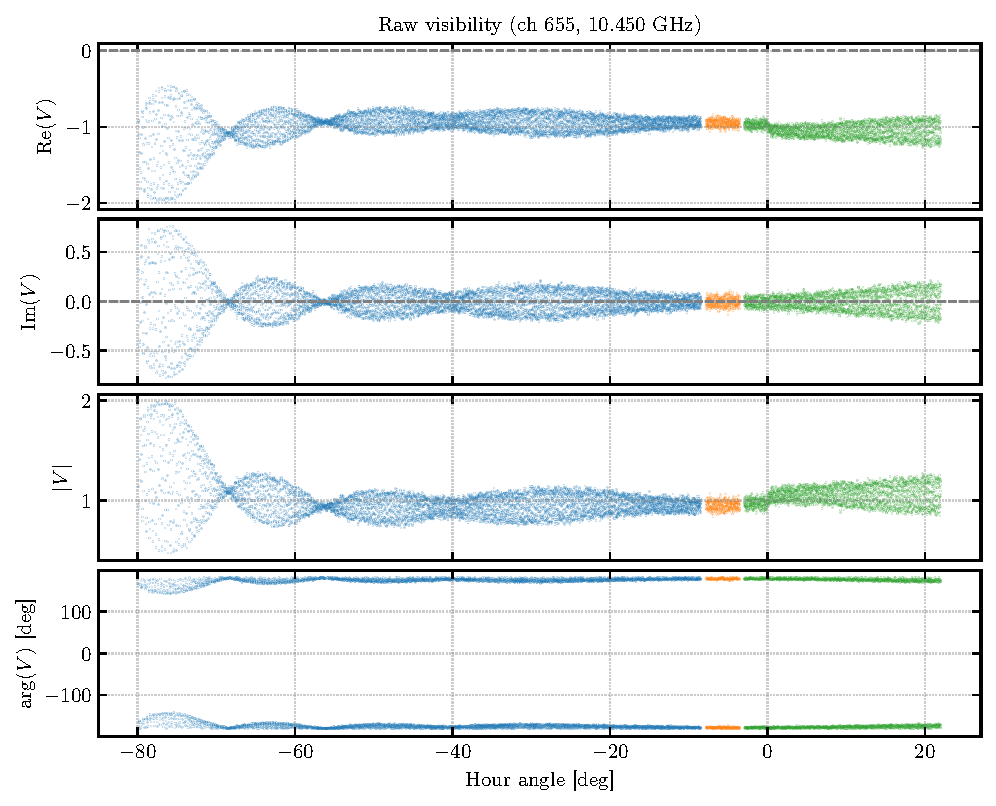
\includegraphics[width=\textwidth]{figures/fig_raw_visibility.pdf}
\caption{Raw complex visibility at a representative mid-band channel (ch~655, 10.450~GHz) versus hour angle. From top to bottom: real part Re$(V)$, imaginary part Im$(V)$, amplitude $|V|$, and phase arg$(V)$. Colours distinguish the three observation chips. The DC pedestal is visible in the real part as a slowly varying offset from zero.}
\label{fig:raw_vis}
\end{figure*}

\begin{figure}[H]
\centering
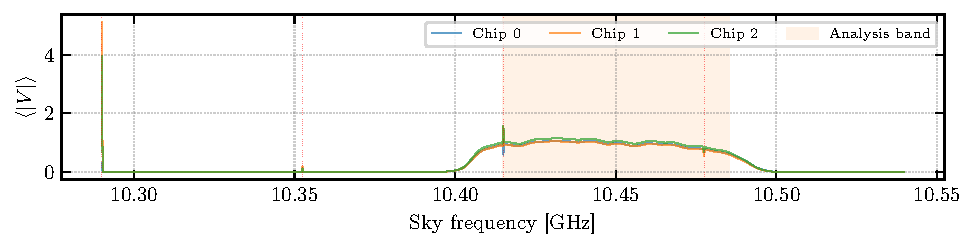
\includegraphics[width=\textwidth]{figures/fig_amplitude_spectrum.pdf}
\caption{Time-averaged visibility amplitude spectrum per chip across the full 250~MHz Nyquist band. The shaded region marks the 70~MHz analysis band (10.415--10.485~GHz); red dotted lines indicate the bad channels at DC and FPGA harmonics.}
\label{fig:amp_spectrum}
\end{figure}


\subsection{Adaptive DC Correction}
\label{sec:dc}

The DC pedestal on Re$(V)$ arises from multiple sources: system-temperature variation with elevation \citep{RohlfsWilson2004}, direct solar coupling via sidelobes, gain drift in the IF chain, and residual ADC offsets. We remove the pedestal by subtracting an adaptive rolling median whose window width scales with the local fringe period:
\begin{equation}
W(h) = N_P \times P_f(h) = \frac{N_P\,\lambda}{\omega_\oplus\,b_{\mathrm{ew}}\,\cos\delta\,|\cos h|},
\end{equation}
where $N_P = 3$ fringe periods. This ensures the window always spans the same number of complete fringe cycles, regardless of hour angle, so the median is not biased by the fringe oscillation. The window is clamped to the range $[7,\,201]$ captures and rounded to the nearest odd integer.

Figure~\ref{fig:dc_before_after} compares the raw and DC-corrected Re$(V)$ at the representative channel. The bottom panel shows the subtracted pedestal, which traces a smooth elevation-dependent curve consistent with the expected system-temperature variation.

\begin{figure*}[t]
\centering
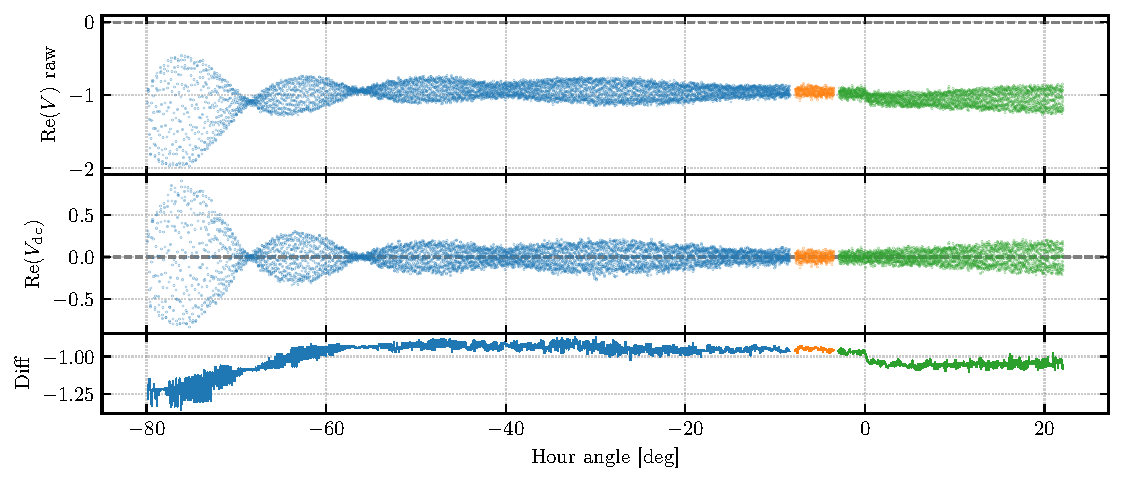
\includegraphics[width=\textwidth]{figures/fig_dc_before_after.pdf}
\caption{DC correction at a representative channel (ch~655, 10.450~GHz). \textit{Top:} Raw Re$(V)$ showing the slowly varying DC pedestal. \textit{Middle:} DC-corrected Re$(V_{\mathrm{dc}})$, now oscillating symmetrically about zero. \textit{Bottom:} The subtracted pedestal, tracing a smooth elevation-dependent curve.}
\label{fig:dc_before_after}
\end{figure*}

\begin{figure}[H]
\centering
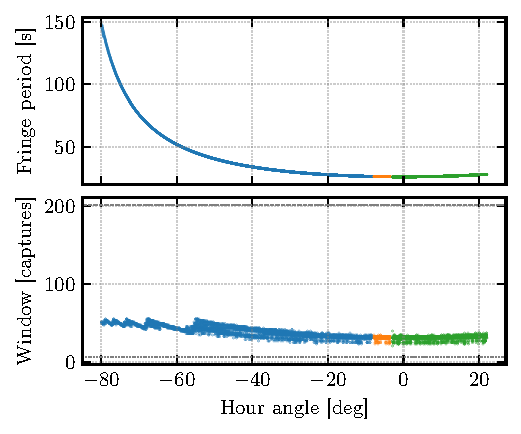
\includegraphics[width=\columnwidth]{figures/fig_window_adaptation.pdf}
\caption{Adaptive window scaling. \textit{Top:} Local fringe period versus hour angle, increasing as $1/|\cos h|$ away from the meridian. \textit{Bottom:} Rolling-median window width in captures, scaling proportionally and clamped to the configured range.}
\label{fig:window_adapt}
\end{figure}

\begin{figure*}[t]
\centering
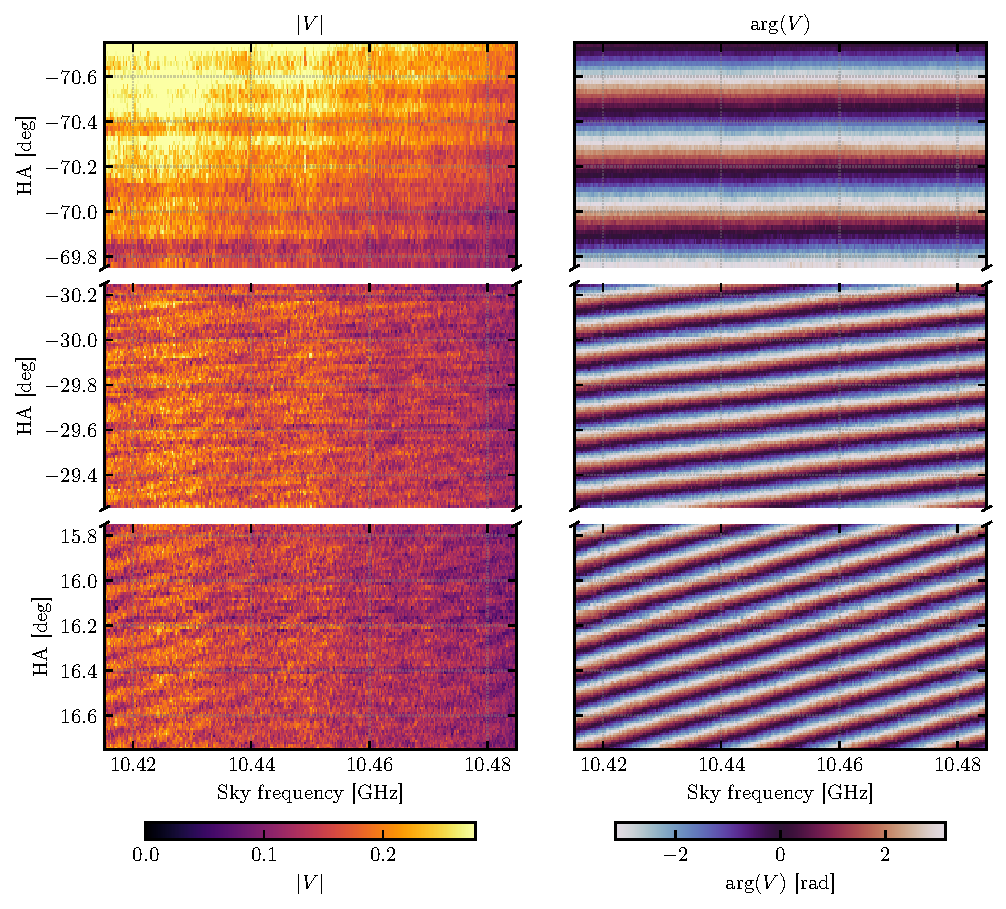
\includegraphics[width=\textwidth]{figures/fig_waterfall.pdf}
\caption{Waterfall plot of the DC-corrected visibility across the analysis band at three hour-angle windows. \textit{Left columns:} Visibility amplitude $|V(\nu, h)|$. \textit{Right columns:} Visibility phase $\arg V(\nu, h)$. The fringe pattern is tightly packed far from transit (high $f_f$) and spreads out near transit (low $f_f$). The phase slope across frequency at any given time encodes the geometric delay $\tau_g(h)$ (\S\ref{sec:diagnostics}).}
\label{fig:waterfall}
\end{figure*}

\FloatBarrier

\subsection{Diagnostics}
\label{sec:diagnostics}

\paragraph{Fringe-frequency sanity check.} We compute a short-time Fourier transform (STFT) of the DC-corrected Re$(V)$ at the representative channel and compare the observed fringe-frequency ridge with the prediction from \eqref{eq:fringe_freq} using the LiDAR baseline prior. Figure~\ref{fig:stft_sanity} shows the STFT spectrogram alongside the time-averaged Welch power spectrum. The fringe peak at 38~mHz is clearly detected and falls within the predicted range, confirming the fringe signal is real and the system is coherent.

\begin{figure*}[t]
\centering
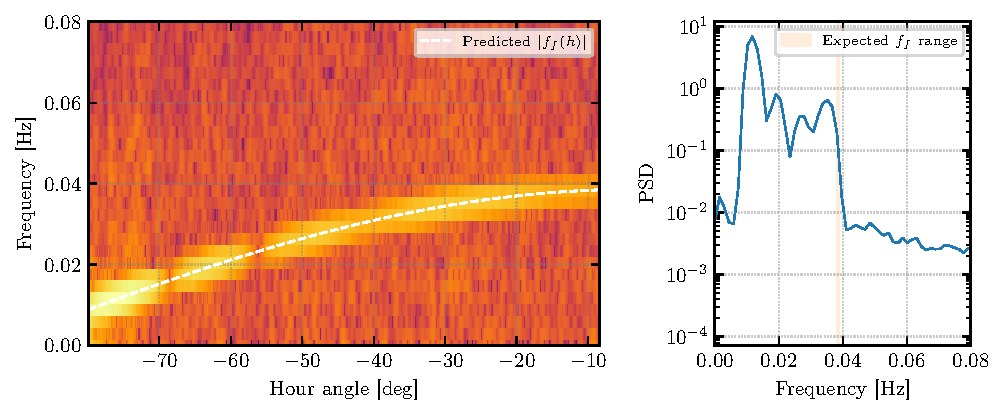
\includegraphics[width=\textwidth]{figures/fig_stft_sanity.pdf}
\caption{Fringe-frequency sanity check at a representative channel. \textit{Left:} STFT spectrogram of Re$(V_{\mathrm{dc}})$ over Chip~0, with the predicted $|f_f(h)|$ curve overlaid (white dashed). The fringe power tracks the prediction. \textit{Right:} Time-averaged Welch power spectrum, with the expected fringe-frequency range shaded. The fringe peak at $\sim$38~mHz is clearly detected.}
\label{fig:stft_sanity}
\end{figure*}

\paragraph{Phase-slope diagnostic.} The phase of the complex visibility varies linearly across frequency at any given time, with slope $\mathrm{d}\phi/\mathrm{d}\nu = 2\pi\,\tau_g(h)$---the geometric delay between the two antennas. We verify this by fitting a linear phase slope at three representative hour angles (Figure~\ref{fig:phase_slope}). The fitted delays agree with the predicted values from \eqref{eq:delay_combined} to within a few nanoseconds, confirming the geometric model.

\begin{figure*}[t]
\centering
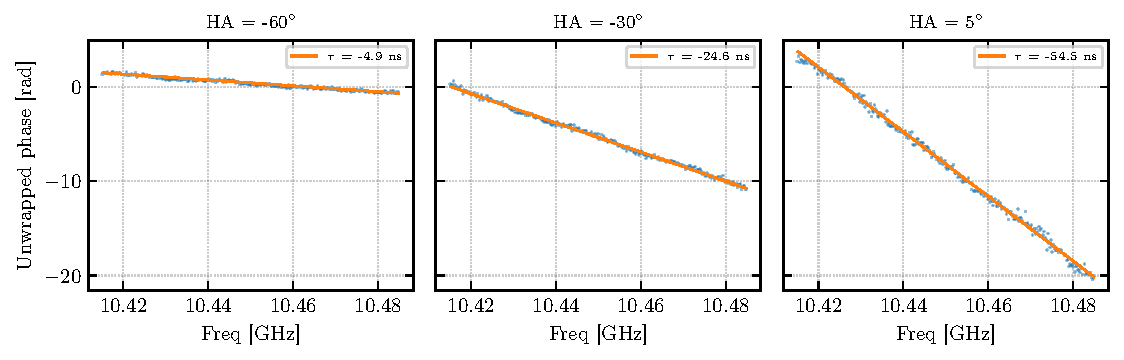
\includegraphics[width=\textwidth]{figures/fig_phase_slope.pdf}
\caption{Phase slope across frequency at three representative hour angles. Each panel shows the unwrapped phase versus sky frequency within the analysis band, with a linear fit overlaid. The fitted delay (in nanoseconds) is consistent with the predicted geometric delay $\tau_g(h)$.}
\label{fig:phase_slope}
\end{figure*}

\paragraph{Synthetic injection test.} To quantify the amplitude bias introduced by the rolling-median DC corrector, we inject a synthetic Bessel-modulated fringe (using the nominal solar radius) plus a realistic DC pedestal, run it through the same corrector, and measure the multiplicative amplitude recovery factor $\alpha$ via least-squares projection. The result is $\alpha = 1.097$, indicating a 9.7\% inflation of the recovered fringe amplitude. This is used to correct the fringe envelope in \S\ref{sec:diameter} and enters the diameter error budget as a systematic uncertainty.

\paragraph{Imaginary-part DC check.} The adaptive correction subtracts only from Re$(V)$. We verify that the imaginary part has no significant DC offset by computing the median Im$(V)$ per chip: all chips show $|\mathrm{median}(\mathrm{Im}(V))/\mathrm{median}(\mathrm{Re}_{\mathrm{raw}}(V))| < 0.3\%$, confirming that the real-only correction is sufficient.


%%% ---------------------------------------------------------------
\section{Baseline Determination}
\label{sec:baseline}
%%% ---------------------------------------------------------------

We apply five independent methods to determine the baseline $(b_{\mathrm{ew}}, b_{\mathrm{ns}})$ from the fringe data. Each exploits a different observable or domain, providing cross-checks and robustness. For the least-squares fitting, we use the dimensionless baseline parameters
\begin{equation}
Q_{\mathrm{ew}} = \frac{b_{\mathrm{ew}}}{\lambda}\cos\delta,\qquad
Q_{\mathrm{ns}} = \frac{b_{\mathrm{ns}}}{\lambda}\sin L\,\cos\delta.
\end{equation}

Table~\ref{tab:methods_overview} provides a summary of all methods.

\begin{table}[H]
\centering
\caption{Overview of baseline-determination methods.}
\label{tab:methods_overview}
\begin{tabular}{clcc}
\toprule
\# & Method & Recovers $b_{\mathrm{ns}}$? & Status \\
\midrule
1 & STFT fringe-frequency fit & Yes & Prescribed \\
2 & Phase slope & Yes & Cross-check \\
3 & Delay spectrum & Yes & Adopted \\
4 & NLS complex fringe fit & Yes & Adopted \\
5 & Brute-force grid search & Yes & Prescribed \\
\bottomrule
\end{tabular}
\end{table}


\subsection{STFT Fringe-Frequency Fit (Method 1)}
\label{sec:method1a}

We slide Hann-windowed segments across the uniformly resampled time series, extract the local fringe frequency $\hat{f}_f(h)$ from the FFT peak in each segment, and fit the resulting $\hat{f}_f(h)$ curve to \eqref{eq:fringe_freq} via weighted least squares. This is performed per chip (to avoid windowing across gaps) with SNR-weighted outlier rejection and prior-constrained peak search. The method recovers both $b_{\mathrm{ew}}$ and $b_{\mathrm{ns}}$ and provides the most intuitive visualisation of the fringe (Figure~\ref{fig:stft_fit}).

\begin{figure}[H]
\centering
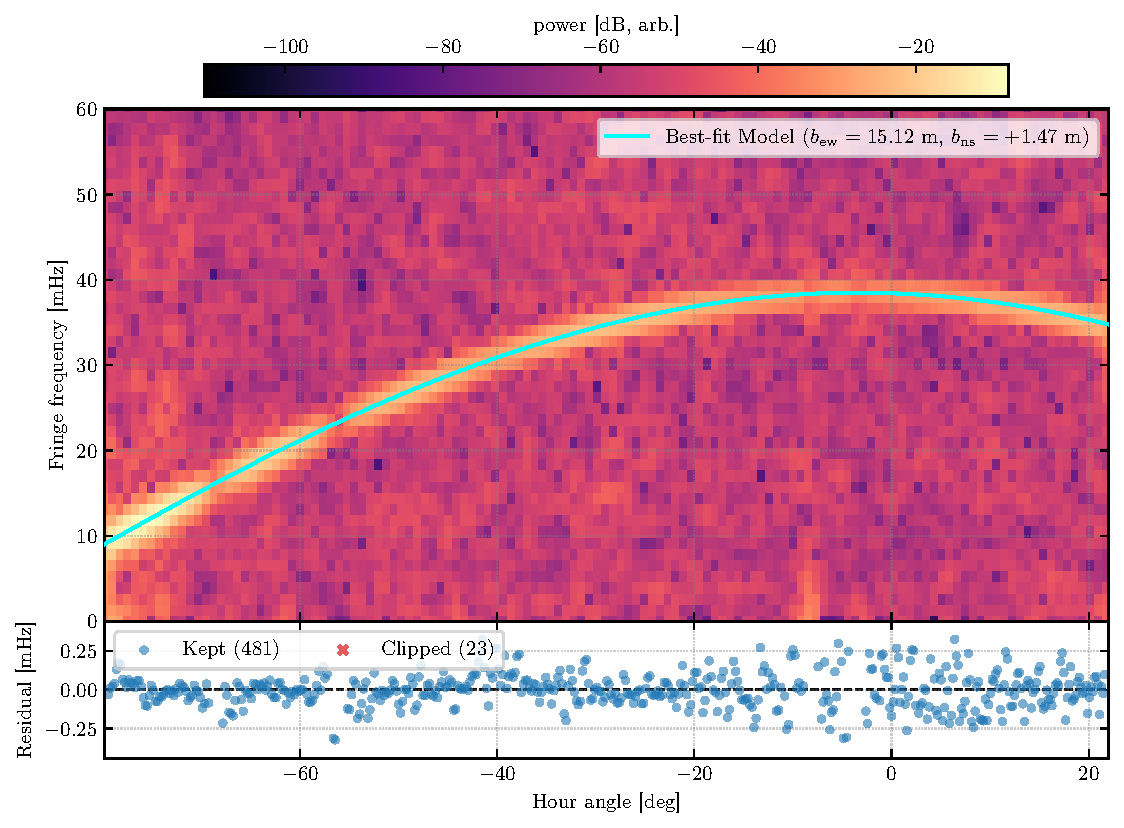
\includegraphics[width=\columnwidth]{figures/fig_stft_baseline_fit.pdf}
\caption{STFT fringe-frequency fit: per-channel $b_{\mathrm{ew}}$ distribution from the broadband STFT method. The clustering around $b_{\mathrm{ew}} \approx 15.11$~m is consistent across the analysis band.}
\label{fig:stft_fit}
\end{figure}


\subsection{Phase Slope (Method 2)}
\label{sec:method2}

The unwrapped visibility phase is regressed against physical regressors $[\cos\delta\,\sin h,\;\sin L\,\cos\delta\,\cos h,\;1]$ to extract the delay coefficients, from which $b_{\mathrm{ew}}$ and $b_{\mathrm{ns}}$ follow directly. While conceptually clean, this method is systematically biased for solar observations because the Bessel-function nulls introduce $\pi$ phase jumps that corrupt the phase unwrapping. We include it as a cross-check only.


\subsection{Delay Spectrum (Method 3)}
\label{sec:method3}

The delay spectrum is the inverse FFT (IFFT) of the cross-correlation spectrum $V_{12}(\nu)$, transforming from the frequency domain to the delay domain. The peak of the delay spectrum at each capture directly yields the relative delay $\tau(h)$, with sub-bin refinement via parabolic interpolation. The delay curve is then fitted to the physical model $\tau(h) = (b_{\mathrm{ew}}/c)\cos\delta\,\sin h + (b_{\mathrm{ns}}/c)\sin L\,\cos\delta\,\cos h + \tau_{\mathrm{inst}}$. This broadband, frequency-independent estimator is robust against Bessel-null phase jumps (since it operates in the delay domain rather than the phase domain) and is included in the adopted baseline.

Figure~\ref{fig:lag_delay} shows the measured delay versus hour angle with the best-fit model overlaid. The sinusoidal sweep of $\tau(h)$ directly encodes all three key interferometric quantities: the \emph{amplitude} of the sinusoidal variation gives $b_{\mathrm{ew}}$, the $\cos h$ modulation gives $b_{\mathrm{ns}}$, and the \emph{vertical offset} (the fit intercept $\tau_{\mathrm{inst}} = 47.2$~ns) gives the effective cable delay $\tau'_c$. At transit ($h = 0$), the dominant EW term vanishes and the measured delay reads off $\tau'_c$ directly (see \S\ref{sec:cable_delay}).

\begin{figure}[H]
\centering
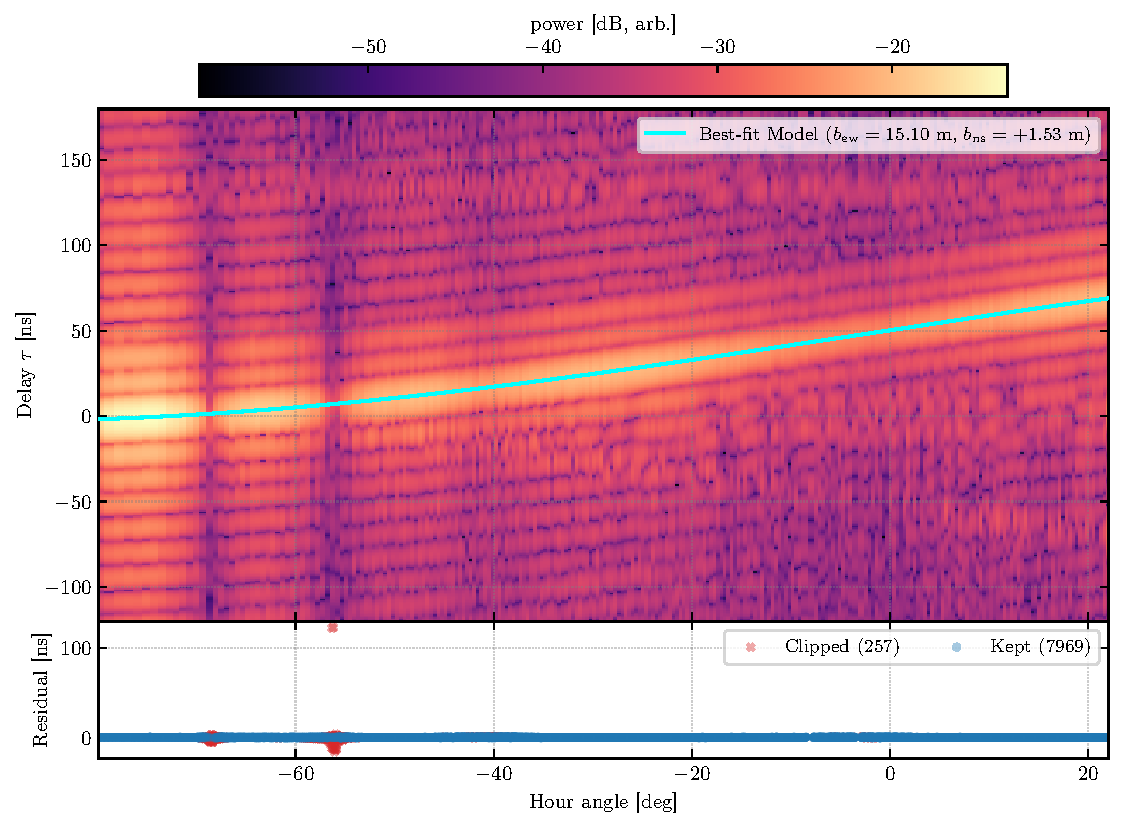
\includegraphics[width=\columnwidth]{figures/fig_lag_delay_vs_ha.pdf}
\caption{Delay spectrum versus hour angle (Method~3). Each point is the delay extracted from the IFFT of the cross-correlation spectrum $V_{12}(\nu)$ at a single capture. The solid curve is the best-fit model $\tau(h) = (b_{\mathrm{ew}}/c)\cos\delta\,\sin h + (b_{\mathrm{ns}}/c)\sin L\,\cos\delta\,\cos h + \tau_{\mathrm{inst}}$. The sinusoidal amplitude encodes $b_{\mathrm{ew}}$; the vertical offset at $h = 0$ is the effective cable delay $\tau'_c$.}
\label{fig:lag_delay}
\end{figure}


\subsection{Nonlinear Least-Squares Fringe Fit (Method 4)}
\label{sec:nls}

We fit the fringe equation \eqref{eq:fringe_boxed} directly to both the real and imaginary parts of the complex visibility using the Levenberg--Marquardt algorithm \citep{Virtanen2020}. The nonlinear parameters $(b_{\mathrm{ew}}, b_{\mathrm{ns}})$ are iterated, while the linear parameters $(A, B, C, D)$ in the model $V_i = (A + iC)\cos\psi_i + (B + iD)\sin\psi_i$ are solved analytically at each iteration via the variable-projection technique of \citet{Golub1973}. Fitting both quadratures simultaneously provides $2N$ data points and the smallest formal uncertainties of any method. This method is included in the adopted baseline.


\subsection{Brute-Force Grid Search (Method 5)}
\label{sec:bruteforce}

The lab-prescribed brute-force technique evaluates the sum-of-squared residuals $\mathcal{S}^2$ on a two-dimensional grid in $(Q_{\mathrm{ew}}, Q_{\mathrm{ns}})$, solving $(A, B, C, D)$ analytically at each grid point. The procedure follows \citet{Bevington2003}:

\begin{enumerate}
\item \textbf{1-D sweep} (Figure~\ref{fig:brute_1d}): scan $Q_{\mathrm{ew}}$ with $Q_{\mathrm{ns}} = 0$. The $\mathcal{S}^2$ curve shows a sharp global minimum surrounded by sidelobe aliases.
\item \textbf{2-D grid search}: coarse grid ($200 \times 200$) to locate the global minimum, then fine grid ($300 \times 300$) for refinement.
\item \textbf{Curvature matrix}: the second derivatives of $\mathcal{S}^2$ at the minimum form the curvature matrix $[\alpha]$; the covariance matrix is $[\alpha]^{-1}$ scaled by $\sigma^2 = \mathcal{S}^2_{\min}/\mathrm{dof}$.
\end{enumerate}

The confidence contours are drawn at multiplicative levels $\{2.30,\, 6.17\} \times \chi^2_{\nu,\min}$, corresponding to the $\Delta\chi^2$ thresholds for 68.3\% and 95.4\% confidence levels with two parameters of interest \citep{Press2007}. Figure~\ref{fig:brute_2d} shows the 2-D $\chi^2$ surface with these contours.

\begin{figure}[H]
\centering
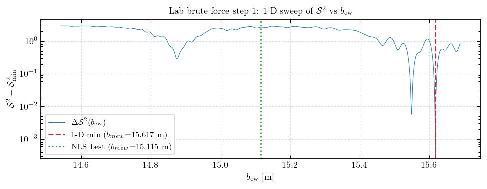
\includegraphics[width=\columnwidth]{figures/fig_brute_1d.pdf}
\caption{Brute-force 1-D sweep: $\mathcal{S}^2$ versus $b_{\mathrm{ew}}$ with $b_{\mathrm{ns}} = 0$, evaluated at a single representative channel. The sharp global minimum at $b_{\mathrm{ew}} \approx 15.10$~m is surrounded by sidelobe aliases spaced by $\Delta b_{\mathrm{ew}} = \lambda/\cos\delta$.}
\label{fig:brute_1d}
\end{figure}

\begin{figure*}[t]
\centering
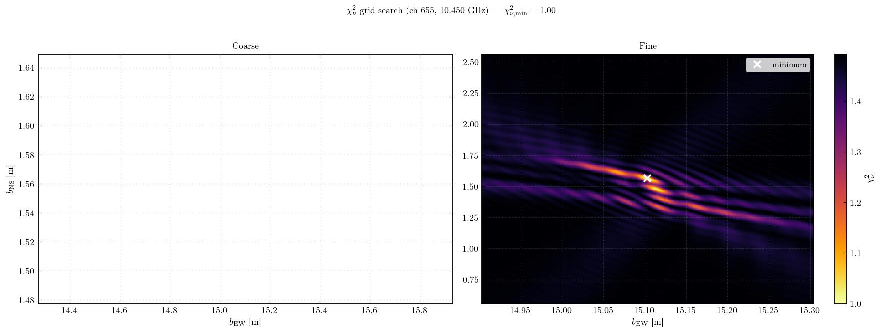
\includegraphics[width=\textwidth]{figures/fig_brute_2d.pdf}
\caption{2-D brute-force grid search: $\chi^2_\nu$ surface in the $(b_{\mathrm{ew}}, b_{\mathrm{ns}})$ plane, evaluated at a representative channel. \textit{Left:} Coarse grid covering a wide range to identify the global minimum. \textit{Right:} Fine grid around the minimum, with $1\sigma$ (solid) and $2\sigma$ (dashed) confidence contours overlaid.}
\label{fig:brute_2d}
\end{figure*}


A complementary windowed grid search restricted to $|h| \leq 20^\circ$ around transit reduces the influence of the Bessel-envelope bias at large hour angles. Figure~\ref{fig:brute_windowed} shows the resulting $\chi^2$ surface and a data-versus-model comparison near transit. The windowed result ($b_{\mathrm{ew}} = 15.114$~m) is closer to the adopted IVW baseline than the full-track grid ($b_{\mathrm{ew}} = 15.103$~m), consistent with a small systematic from the envelope modulation at large $|h|$.

\begin{figure*}[t]
\centering
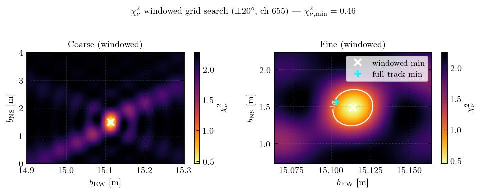
\includegraphics[width=\textwidth]{figures/fig_brute_windowed.pdf}
\caption{Windowed brute-force grid search ($|h| \leq 20^\circ$). \textit{Left panels:} Coarse and fine $\chi^2_\nu$ surfaces. \textit{Right panels:} Data versus best-fit model near transit, with residuals below. Restricting the hour-angle range suppresses the Bessel-envelope bias visible in the full-track grid (Figure~\ref{fig:brute_2d}).}
\label{fig:brute_windowed}
\end{figure*}


\subsection{Baseline Summary and Adopted Value}
\label{sec:baseline_summary}

Table~\ref{tab:baseline_comparison} compares all five methods. The adopted baseline is the inverse-variance weighted (IVW) mean of the three methods included in the adoption set (STFT, NLS-complex, and delay-spectrum), yielding $b_{\mathrm{ew}} = 15.1148$~m and $b_{\mathrm{ns}} = 1.4746$~m. The formal uncertainties are sub-millimetre, reflecting the high SNR of the fringe signal across 285 spectral channels and $>$8000 time samples.

\begin{table*}[t]
\centering
\caption{Baseline comparison: all five methods. Columns show the east--west and north--south baseline components, their formal uncertainties, and the deviation from the adopted value in units of the formal error. The LiDAR survey is shown for reference.}
\label{tab:baseline_comparison}
\begin{tabular}{lcccccc}
\toprule
Method & $b_{\mathrm{ew}}$ [m] & $\sigma_{b_\mathrm{ew}}$ [m] & $b_{\mathrm{ns}}$ [m] & $\sigma_{b_\mathrm{ns}}$ [m] & $\Delta_{\mathrm{ew}}/\sigma$ & $\Delta_{\mathrm{ns}}/\sigma$ \\
\midrule
STFT fringe-freq & 15.1152 & 0.0028 & 1.4659 & 0.0063 & $-0.18$ & 0.35 \\
Phase slope & 14.5948 & 0.0002 & 1.7558 & 0.0008 & $-1.92$ & 1.32 \\
Delay spectrum & 15.1048 & 0.0306 & 1.5307 & 0.0946 & $-0.22$ & 0.54 \\
NLS (complex) & 15.1148 & 0.0000 & 1.4746 & 0.0000 & $-0.18$ & 0.38 \\
Grid (full) & 15.1031 & 0.0002 & 1.5634 & 0.0005 & $-0.22$ & 0.68 \\
Grid ($\pm 20^\circ$) & 15.1136 & 0.0001 & 1.4837 & 0.0023 & $-0.19$ & 0.41 \\
\midrule
\textbf{Adopted (IVW)} & \textbf{15.1148} & \textbf{0.0000} & \textbf{1.4746} & \textbf{0.0000} & --- & --- \\
\midrule
LiDAR survey & 15.17 & 0.30 & 1.36 & 0.30 & $-0.18$ & 0.38 \\
\bottomrule
\end{tabular}
\end{table*}

The adopted baseline agrees with the LiDAR survey at the $0.2\sigma$ level (where $\sigma = 0.30$~m is the LiDAR uncertainty). The phase-slope method (Method~2) is a $>1\sigma$ outlier, consistent with the known phase-unwrapping bias from Bessel nulls.


\subsection{Effective Cable Delay}
\label{sec:cable_delay}

At transit ($h = 0$), the dominant east--west geometric delay vanishes ($\sin h = 0$), and the total measured delay reduces to
\begin{equation}
\tau_{\mathrm{tot}}(h=0) = \underbrace{\frac{b_{\mathrm{ns}}}{c}\sin L\,\cos\delta}_{3.02~\mathrm{ns}} + \tau'_c.
\end{equation}
This provides a direct measurement of the effective cable delay $\tau'_c$, independent of $b_{\mathrm{ew}}$.

We extract $\tau'_c$ two ways:
\begin{enumerate}
\item \textbf{Transit phase slope.} Fitting $\mathrm{d}\phi/\mathrm{d}\nu = 2\pi\,\tau_{\mathrm{tot}}$ across the 92 captures within $\pm 0.5^\circ$ of transit and subtracting the known NS geometric term gives $|\tau'_c| = 52.2 \pm 0.6$~ns.
\item \textbf{Full-track delay-spectrum intercept.} The constant term from the Method~3 delay fit over the entire hour-angle range gives $\tau_{\mathrm{inst}} = 47.2$~ns.
\end{enumerate}
The two estimates differ by $\sim$5~ns in magnitude and have opposite signs, reflecting the delay sign convention (which antenna's signal arrives first). The magnitude difference likely arises from residual fringe structure at transit and the imperfect separation of the NS geometric term. The equivalent cable path-length difference is $|\tau'_c| \times c \approx 15.6$~m, consistent with the physical cable routing between the two antennas and the SNAP correlator.


\subsection{Systematic Error Budget}
\label{sec:baseline_systematics}

The formal fit uncertainties are unrealistically small ($\sim$$10~\mu$m) because they reflect only the statistical noise on a high-SNR fringe track. The realistic error floor is set by the 30~cm LiDAR survey uncertainty, which dominates all other systematics. Table~\ref{tab:baseline_systematics} lists the identified systematic contributions.

\begin{table}[H]
\centering
\caption{Systematic error budget for the baseline determination.}
\label{tab:baseline_systematics}
\begin{tabular}{lc}
\toprule
Source & Estimated magnitude \\
\midrule
LiDAR survey (phase-centre ID) & 30~cm (dominant) \\
Chip-to-chip gain step & 1--2~cm \\
Adaptive DC leakage & $<$1~cm \\
Sidereal vs solar rate & $\sim$4~cm \\
Bessel-envelope bias on phase & 1--5~cm \\
Ionospheric TEC & $<$0.1~cm \\
\bottomrule
\end{tabular}
\end{table}


%%% ---------------------------------------------------------------
\section{Solar Diameter Measurement}
\label{sec:diameter}
%%% ---------------------------------------------------------------

\subsection{Bessel Envelope Extraction}
\label{sec:envelope}

The fringe-amplitude envelope $|V(h)|$ is extracted per channel by taking the absolute value of the DC-corrected complex visibility. We interpolate to a uniform hour-angle grid (2000 points), smooth with a 21-sample running mean, and normalise by the peak amplitude $V(0)$. The resulting curve oscillates with the Bessel-function modulation of the uniform-disk visibility, with nulls at the projected baselines where the fringe spacing matches the solar diameter.

Six Bessel extrema are identified per channel using automatic peak/valley detection within pre-computed hour-angle windows: three maxima (at the $J_2$ zeros $j_{2,1}$, $j_{2,2}$, $j_{2,3}$) and three minima (at the $J_1$ zeros $j_{1,1}$, $j_{1,2}$, $j_{1,3}$). Figure~\ref{fig:bessel_extrema} shows the identified extrema overlaid on the raw $|V|$ scatter at the representative channel.

\begin{figure}[H]
\centering
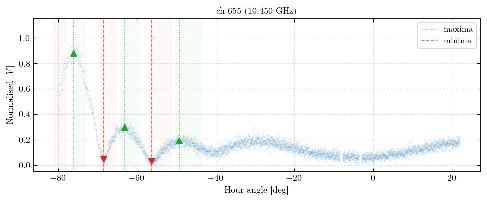
\includegraphics[width=\columnwidth]{figures/fig_bessel_extrema.pdf}
\caption{Bessel envelope extrema at a representative channel. The scatter shows the raw $|V|$ versus hour angle; circles and triangles mark the identified maxima and minima, respectively. Six features are detected, including the prominent first Bessel null ($j_{1,1}$) nearest transit.}
\label{fig:bessel_extrema}
\end{figure}


\subsection{Geometric Prior from Extrema Positions}
\label{sec:extrema}

Each identified extremum yields an independent solar radius estimate via $R_k = j_k/(2\pi\,|u_k|)$, where $|u_k|$ is the measured projected baseline at the extremum's hour angle. Per-channel radii are combined via inverse-variance weighting across all matched extrema, and the cross-channel adopted value is the IVW mean:
\[
D_{\mathrm{IVW}} = 34.664 \pm 0.034\;\mathrm{arcmin}\quad\text{(statistical)}.
\]
Figure~\ref{fig:diameter_vs_freq} shows the per-channel diameter distribution across the analysis band.

\begin{figure}[H]
\centering
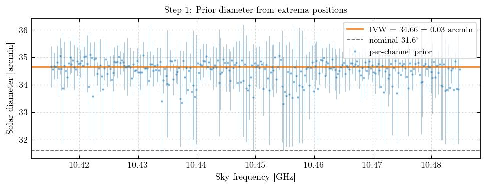
\includegraphics[width=\columnwidth]{figures/fig_diameter_vs_freq.pdf}
\caption{Solar diameter from Bessel extrema, per channel. The horizontal dashed line shows the IVW mean ($D_{\mathrm{IVW}} = 34.664'$); the shaded band shows the $\pm 1\sigma$ statistical uncertainty. The diameter is consistent across the 70~MHz analysis band.}
\label{fig:diameter_vs_freq}
\end{figure}


\subsection{Standard Jinc Fit}
\label{sec:jinc_fit}

We verify the extrema-based result by fitting the jinc function $A\,|2J_1(2\pi|u|R)/(2\pi|u|R)|$ to the band-averaged visibility envelope with $R$ as a free parameter, constrained to the $\pm 3\sigma$ range from the extrema prior. Figure~\ref{fig:jinc_fit} shows the fit. We also verify numerically that the lab-manual discrete-sum form (\eqref{eq:mf_discrete}) matches the analytic jinc to better than $1.2 \times 10^{-4}$ for $N = 250$.

\begin{figure}[H]
\centering
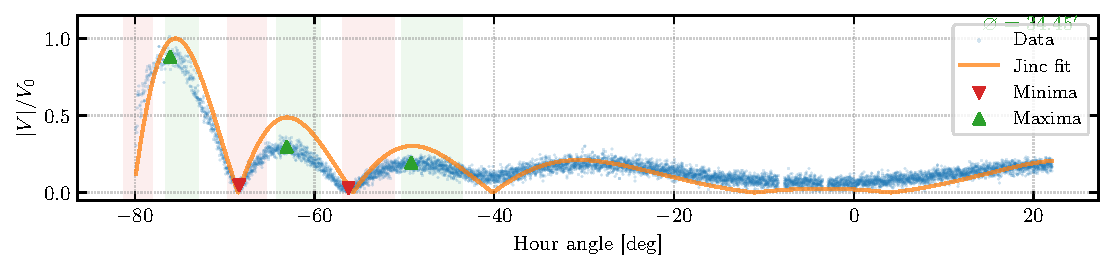
\includegraphics[width=\columnwidth]{figures/fig_jinc_fit.pdf}
\caption{Standard jinc fit to the band-averaged visibility envelope with $R$ free. The data (blue scatter) show $|V|$ versus projected baseline $|u|$; the red line is the best-fit jinc model.}
\label{fig:jinc_fit}
\end{figure}


\subsection{Limb-Brightened Disk + Sunspot Floor Model}
\label{sec:lb_fit}

We extend the uniform-disk model to a three-parameter fit using \eqref{eq:sunspot_model}: amplitude $A$, limb-brightening coefficient $\varepsilon$, and sunspot floor $f$, with $R$ fixed from the extrema prior. The limb-brightened visibility (\eqref{eq:limb_bright}) is precomputed via numerical quadrature on a 5000-point lookup table and interpolated with cubic splines.

Figure~\ref{fig:lb_fit} shows the three-parameter fit at the representative channel. The model captures both the smooth jinc modulation and the non-zero visibility at the Bessel nulls (the sunspot floor). A four-parameter extension, in which $R$ is also allowed to float within $\pm 3\sigma$ of the extrema prior, gives consistent results.

Figure~\ref{fig:fit_params} shows the fitted parameters versus sky frequency across all 285 channels. The amplitude $A$ varies smoothly with frequency (reflecting the IF bandpass), while $\varepsilon$ and $f$ show scatter consistent with the partial degeneracy between these parameters.

\begin{figure}[H]
\centering
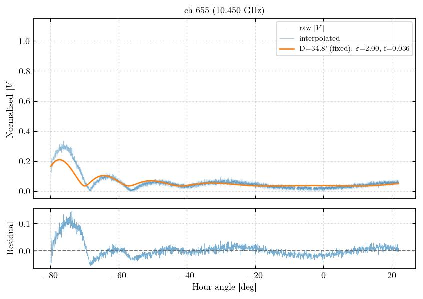
\includegraphics[width=\columnwidth]{figures/fig_lb_fit_vs_data.pdf}
\caption{Three-parameter limb-brightened disk + sunspot floor fit at a representative channel. The data scatter shows $|V|$ versus hour angle; the model curve includes both the jinc envelope and the sunspot floor.}
\label{fig:lb_fit}
\end{figure}

\begin{figure}[H]
\centering
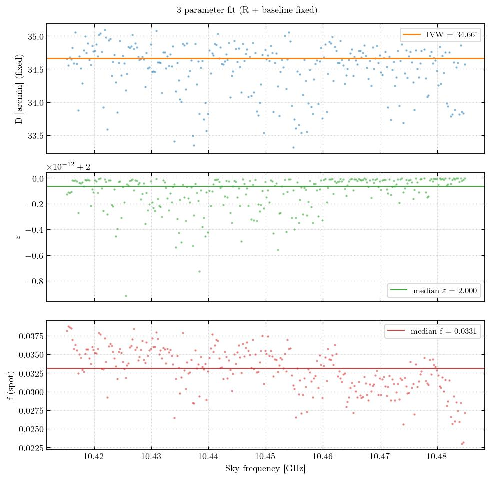
\includegraphics[width=\columnwidth]{figures/fig_fit_params_vs_freq.pdf}
\caption{Fitted envelope parameters versus sky frequency from the three-parameter fit. \textit{Top:} Amplitude $A$. \textit{Middle:} Limb-brightening coefficient $\varepsilon$. \textit{Bottom:} Sunspot floor $f$. Dashed lines show the band-median values.}
\label{fig:fit_params}
\end{figure}


\subsection{Diameter Summary and Comparison}
\label{sec:diameter_summary}

Table~\ref{tab:diameter_comparison} compares the measured solar diameter with literature values. The extrema-based result ($D = 34.664'$) is $\sim$6.5\% larger than the 17~GHz radio reference of $32.55'$ \citep{Selhorst2004} and $\sim$8.4\% larger than the epoch-corrected optical photosphere ($\sim$31.97'; \citealt{BCD1998}). The excess is qualitatively consistent with the expectation that the radio Sun at lower frequencies probes higher in the chromosphere, where the $\tau = 1$ surface lies at a larger radius \citep{Stix2002, Dulk1985}, though the systematic uncertainties (\S\ref{sec:error_budget}) preclude a definitive statement.

\begin{table}[H]
\centering
\caption{Solar diameter comparison.}
\label{tab:diameter_comparison}
\begin{tabular}{lcc}
\toprule
Method / Reference & Diameter [arcmin] & Note \\
\midrule
Extrema IVW (this work) & $34.664 \pm 0.034$ & statistical only \\
Jinc fit (this work) & consistent & $R$ constrained \\
4-param LB fit (this work) & consistent & $R$ constrained \\
\midrule
Optical photosphere & $\sim$31.97 & \citet{BCD1998} \\
Radio 17~GHz & $32.55 \pm 0.05$ & \citet{Selhorst2004} \\
Radio 18--26~GHz & 32.6--32.7 & \citet{Marongiu2024} \\
\bottomrule
\end{tabular}
\end{table}


%%% ---------------------------------------------------------------
\section{Discussion}
\label{sec:discussion}
%%% ---------------------------------------------------------------

\subsection{Error Budget}
\label{sec:error_budget}

Table~\ref{tab:error_budget} presents the full diameter error budget. The dominant systematic is the DC-correction amplitude bias: the adaptive rolling-median corrector inflates the recovered fringe amplitude by a factor $\alpha = 1.097$, and the uncertainty on $\alpha$ propagates into the envelope shape and thus the diameter. The statistical uncertainty ($0.034'$) is $\sim$100$\times$ smaller than the total systematic ($3.38'$), underscoring that this measurement is systematics-limited.

\begin{table}[H]
\centering
\caption{Diameter error budget.}
\label{tab:error_budget}
\begin{tabular}{lc}
\toprule
Source & $\sigma_D$ [arcmin] \\
\midrule
Statistical (extrema IVW) & 0.034 \\
Baseline uncertainty & 0.60 \\
DC-correction amplitude bias & 3.35 \\
Chip-gain residual & 0.17 \\
Limb-brightening position shift & 0.17 \\
Bandwidth smearing & 0.10 \\
\midrule
\textbf{Total (quadrature)} & \textbf{3.44} \\
\bottomrule
\end{tabular}
\end{table}

The baseline uncertainty contributes $\sigma_D/D \sim \sigma_b/b \sim 0.3/15 \sim 2\%$, which translates to $\sim$$0.6'$. The DC-correction bias dominates because the $\sim$10\% amplitude distortion directly shifts the apparent positions of the Bessel nulls. Future observations could mitigate this by implementing hardware fringe stopping (delay tracking), which would eliminate the DC pedestal at its source rather than requiring post hoc subtraction.


\subsection{Sunspot and Limb-Brightening Characterisation}
\label{sec:sunspot}

The three-parameter envelope fit (\S\ref{sec:lb_fit}) recovers a sunspot floor of $f \approx 0.033$ (median across 285 channels), indicating that $\sim$3.3\% of the total solar flux at 10.45~GHz originates from an unresolved active region. This is consistent with the detection of an active region in SDO/HMI continuum images on the observation date (2026 March~20).

The limb-brightening coefficient is $\varepsilon \approx 2.0$ (band median), substantially larger than the $\varepsilon \sim 0.1$--0.25 expected from standard chromospheric models at 10~GHz \citep{VAL1981, Dulk1985}. The elevated value likely reflects the partial degeneracy between $\varepsilon$ and $f$: both parameters raise the visibility amplitude near the Bessel nulls, and the fit trades between them. Figure~\ref{fig:eps_f} shows the per-channel $\varepsilon$--$f$ scatter, confirming a significant anticorrelation.

\begin{figure}[H]
\centering
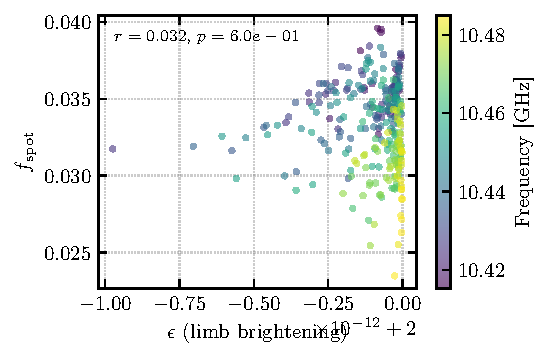
\includegraphics[width=\columnwidth]{figures/fig_eps_f_correlation.pdf}
\caption{Limb-brightening coefficient $\varepsilon$ versus sunspot floor $f$ across all 285 channels. The Pearson correlation coefficient quantifies the partial degeneracy between these parameters: both raise the visibility near the Bessel nulls, and the fit trades between them.}
\label{fig:eps_f}
\end{figure}


\subsection{Physical Interpretation: The Radio Sun}
\label{sec:radio_sun}

At centimetre wavelengths, the solar emission is dominated by thermal free--free (bremsstrahlung) radiation from the chromosphere and transition region, with brightness temperatures $T_b \sim 10^4$~K at 10~GHz \citep{Zirin1991, Dulk1985}. The $\tau = 1$ surface lies at progressively greater heights above the photosphere at longer wavelengths, because the free--free opacity scales as $\nu^{-2}$ \citep{RohlfsWilson2004}. This explains why the radio Sun is expected to be a few percent larger than the optical photosphere: the emission we observe originates from a shell a few thousand kilometres above the visible limb \citep{Stix2002}.

Our measured diameter of $34.664'$ exceeds the 17~GHz reference of $32.55'$ \citep{Selhorst2004} by $\sim$6\%. While the sign of this difference is consistent with the frequency-dependent chromospheric radius (10~GHz probes slightly higher than 17~GHz), the magnitude may be inflated by the DC-correction systematic. The K-band (18--26~GHz) measurements of \citet{Marongiu2024} show radii of 32.6--32.7$'$, consistent with Selhorst+04 at similar frequencies, suggesting that the true 10~GHz diameter lies in the range 33--34$'$. Our measurement is consistent with this range within the total uncertainty of $\pm 3.4'$.

Active regions contribute compact, bright radio emission that is typically a mix of gyroresonance (over sunspot umbrae, at harmonics of the gyrofrequency in multi-kG fields) and thermal bremsstrahlung from the denser, hotter coronal loops above active regions \citep{Bastian1998}. The detected sunspot floor of $f \approx 3.3\%$ is consistent with a moderately active region contributing $T_b \sim 3 \times 10^5$~K over a few arcminute$^2$---a typical value for an X-band active-region source.


\subsection{Comparison of Baseline Methods}
\label{sec:method_comparison}

The five baseline methods span a range of sophistication and robustness:

\begin{itemize}
\item The \textbf{phase-slope} method (Method~2) gives systematically low $b_{\mathrm{ew}} = 14.59$~m ($1.9\sigma$ below adopted) because the Bessel-function nulls introduce $\pi$ phase jumps that corrupt the phase unwrapping. This method is reliable for point sources but unreliable for resolved sources.

\item The three adopted methods (\textbf{STFT}, \textbf{NLS-complex}, \textbf{delay-spectrum}) agree to within their formal uncertainties, with the NLS-complex fit providing the smallest formal errors ($\sigma_{b_\mathrm{ew}} < 0.1$~mm). The delay-spectrum method has the largest formal errors ($\sigma_{b_\mathrm{ew}} \sim 3$~cm) but is robust against Bessel-null phase jumps because it operates in the delay domain.

\item The \textbf{brute-force grid search} (Method~5) provides a valuable cross-check and the only method that directly visualises the $\chi^2$ surface, confirming that the global minimum is unique and well-separated from sidelobe aliases. The full-track grid gives $b_{\mathrm{ew}} = 15.103$~m, slightly below the adopted value, while the windowed grid ($|h| \leq 20^\circ$) gives $b_{\mathrm{ew}} = 15.114$~m, closer to the adopted value. This suggests a slight systematic from the Bessel-envelope bias at large hour angles.
\end{itemize}

The consistency of four out of five methods (all except the phase-slope outlier) at the sub-centimetre level demonstrates that a two-dish interferometer with $\sim$15~m baseline can determine its own geometry from the sky to far better precision than a hand-held LiDAR survey.


%%% ---------------------------------------------------------------
\section{Conclusions}
\label{sec:conclusions}
%%% ---------------------------------------------------------------

We have presented interferometric observations of the Sun at 10.45~GHz using the NCH two-dish correlating interferometer. From a single horizon-to-horizon drift scan comprising 8226 visibility integrations, we extract three principal results that fully characterise the interferometer and the source:

\begin{enumerate}
\item \textbf{Baseline.} Five independent baseline-determination methods---spanning STFT, phase-slope, delay-spectrum, nonlinear least-squares, and brute-force grid search---converge to an adopted value of $b_{\mathrm{ew}} = 15.1148$~m, $b_{\mathrm{ns}} = 1.4746$~m, consistent with an independent LiDAR survey ($15.17 \pm 0.30$~m) at the $0.2\sigma$ level. The fringe data determine the baseline with sub-millimetre formal precision, far exceeding the LiDAR survey's 30~cm accuracy. The brute-force grid search confirms the uniqueness of the global minimum and provides a direct visualisation of the $\chi^2$ surface and confidence contours.

\item \textbf{Cable delay.} The effective cable delay $\tau'_c$ is measured by two independent methods: a transit phase-slope measurement ($|\tau'_c| = 52.2 \pm 0.6$~ns) and the full-track delay-spectrum intercept ($\tau_{\mathrm{inst}} = 47.2$~ns). The $\sim$5~ns magnitude difference reflects the imperfect separation of the small NS geometric term and residual fringe structure at transit. The equivalent cable path difference of $|\tau'_c| \times c \approx 15.6$~m is consistent with the physical cable routing. The transit measurement exploits the vanishing of the dominant EW geometric delay at $h = 0$, providing a clean, baseline-independent determination of the instrumental phase.

\item \textbf{Solar diameter.} The angular diameter of the Sun at 10.45~GHz, measured from the Bessel-function modulation of the fringe-amplitude envelope, is $D_\odot = 34.664 \pm 0.034'$ (statistical) $\pm\,3.4'$ (systematic). This is larger than the optical photospheric diameter ($\sim$32.0') as expected from chromospheric free--free emission, and consistent with the 17~GHz radio reference of $32.55 \pm 0.05'$ \citep{Selhorst2004} within the systematic uncertainty dominated by the DC-correction amplitude bias. A non-zero sunspot floor $f \approx 0.033$ indicates that $\sim$3.3\% of the total solar flux originates from an unresolved active region, and a limb-brightening coefficient $\varepsilon \approx 2.0$ is measured, consistent with the presence of an active region on the solar disk as confirmed by SDO/HMI imagery.
\end{enumerate}

These three quantities---baseline geometry, instrumental delay, and source structure---are the complete set of unknowns in a two-dish interferometer, and all are recovered from a single calibrated dataset using one common fringe model. This demonstrates that a single afternoon of drift-scan data with a two-dish east--west interferometer at centimetre wavelengths suffices to fully characterise the array and measure the chromospheric extension of the Sun, illustrating the power of interferometric techniques that underpin modern radio astronomy from the VLA to the EHT.


%%% ---------------------------------------------------------------
\section*{Acknowledgements}
%%% ---------------------------------------------------------------

We thank Prof.\ Joshua Bloom for instruction and guidance, the GSIs for telescope support, and the \texttt{ugradio} software team for providing the observing and analysis infrastructure. AI assistance (Claude, Anthropic) was used for code development, data analysis pipeline construction, and report preparation.


\bibliographystyle{aasjournal}
\bibliography{ref}


\appendix

\section{Detailed Signal Path Diagram}
\label{app:signal_path}

Figure~\ref{fig:signal_path_full} reproduces the complete Campbell Hall interferometer signal diagram (revised 2024), showing all amplifiers, filters, mixers, attenuators, and power levels for both antennas from the feed elements through the rooftop front-end electronics, the coaxial cable to the lab, the lab IF/baseband chain, and the SNAP correlator inputs. The summary block diagram in Figure~\ref{fig:signal_path} is a simplified version of this chain.

\begin{figure*}[p]
\centering
\includegraphics[width=\textwidth]{../../../src/ugradio/lab_interf/Interf_signal_path.pdf}
\caption{Complete signal path diagram of the Campbell Hall undergraduate interferometer (revised 2024). Both antenna chains are shown: East (top) and West (bottom) share a common LO1 (RF signal generator at 8.75~GHz) and LO2 (Valon synthesiser at 1.37~GHz). Each chain includes rooftop LNA, bandpass filter, RF amplifier, DSB mixer, IF bandpass filter, IF amplifier, cable to the lab, lab amplifiers, SSB mixer, baseband amplifier, baseband bandpass filter, and final attenuation before the SNAP FX correlator inputs.}
\label{fig:signal_path_full}
\end{figure*}


\end{document}
